%%%%%%%%%%%%%%%%%%%%%%%%%%%%%%%%%%%%%%%%%%%%%%%%%%
%% Bachelor's & Master's Thesis Template        %%
%% Copyleft by Dawid Weiss & Marta Szachniuk    %%
%% Faculty of Computing and Telecommunication   %%
%% Poznan University of Technology, 2020        %%
%%%%%%%%%%%%%%%%%%%%%%%%%%%%%%%%%%%%%%%%%%%%%%%%%%


% Szkielet dla pracy licencjackiej pisanej w języku polskim.

\documentclass[english,bachelor,a4paper,oneside]{ppfcmthesis}


\usepackage[utf8]{inputenc}
\usepackage[OT4]{fontenc}

\usepackage{siunitx}
\usepackage{multicol}
\usepackage{pdfpages}

\usepackage{newfloat,caption,float}
\DeclareFloatingEnvironment[placement={!h},name=List]{mylist}
\DeclareFloatingEnvironment[fileext=loe, listname=Examples, name=Example, placement=H, within=none]{example}
\captionsetup[example]{}

\usepackage{listings}
\lstset{
basicstyle=\small\ttfamily,
%xleftmargin=.05\textwidth, xrightmargin=.05\textwidth
}


%--------------------------------------
% Strona tytułowa
%--------------------------------------

% Autorzy pracy, jeśli jest ich więcej niż jeden
% wstaw między nimi separator \and
% w kolejności alfabetycznej
\author{%
   Dariusz Max Adamski \album{136674} \and 
   Sławomir Gilewski \album{142192} \and
   Piotr Jurga \album{136728}
}
\authortitle{}                                % Do not change.

\title{AI Colosseum: a system for automatic evaluation of game playing bots}

% Your supervisor comes here.
\ppsupervisor{dr~inż.~Jędrzej Potoniec} 

% Year of final submission (not graduation!)
\ppyear{2021}                                 


\begin{document}

% Front matter starts here
\frontmatter\pagestyle{empty}%
\maketitle\cleardoublepage%

%--------------------------------------
% Miejsce na kartę pracy dyplomowej
%--------------------------------------

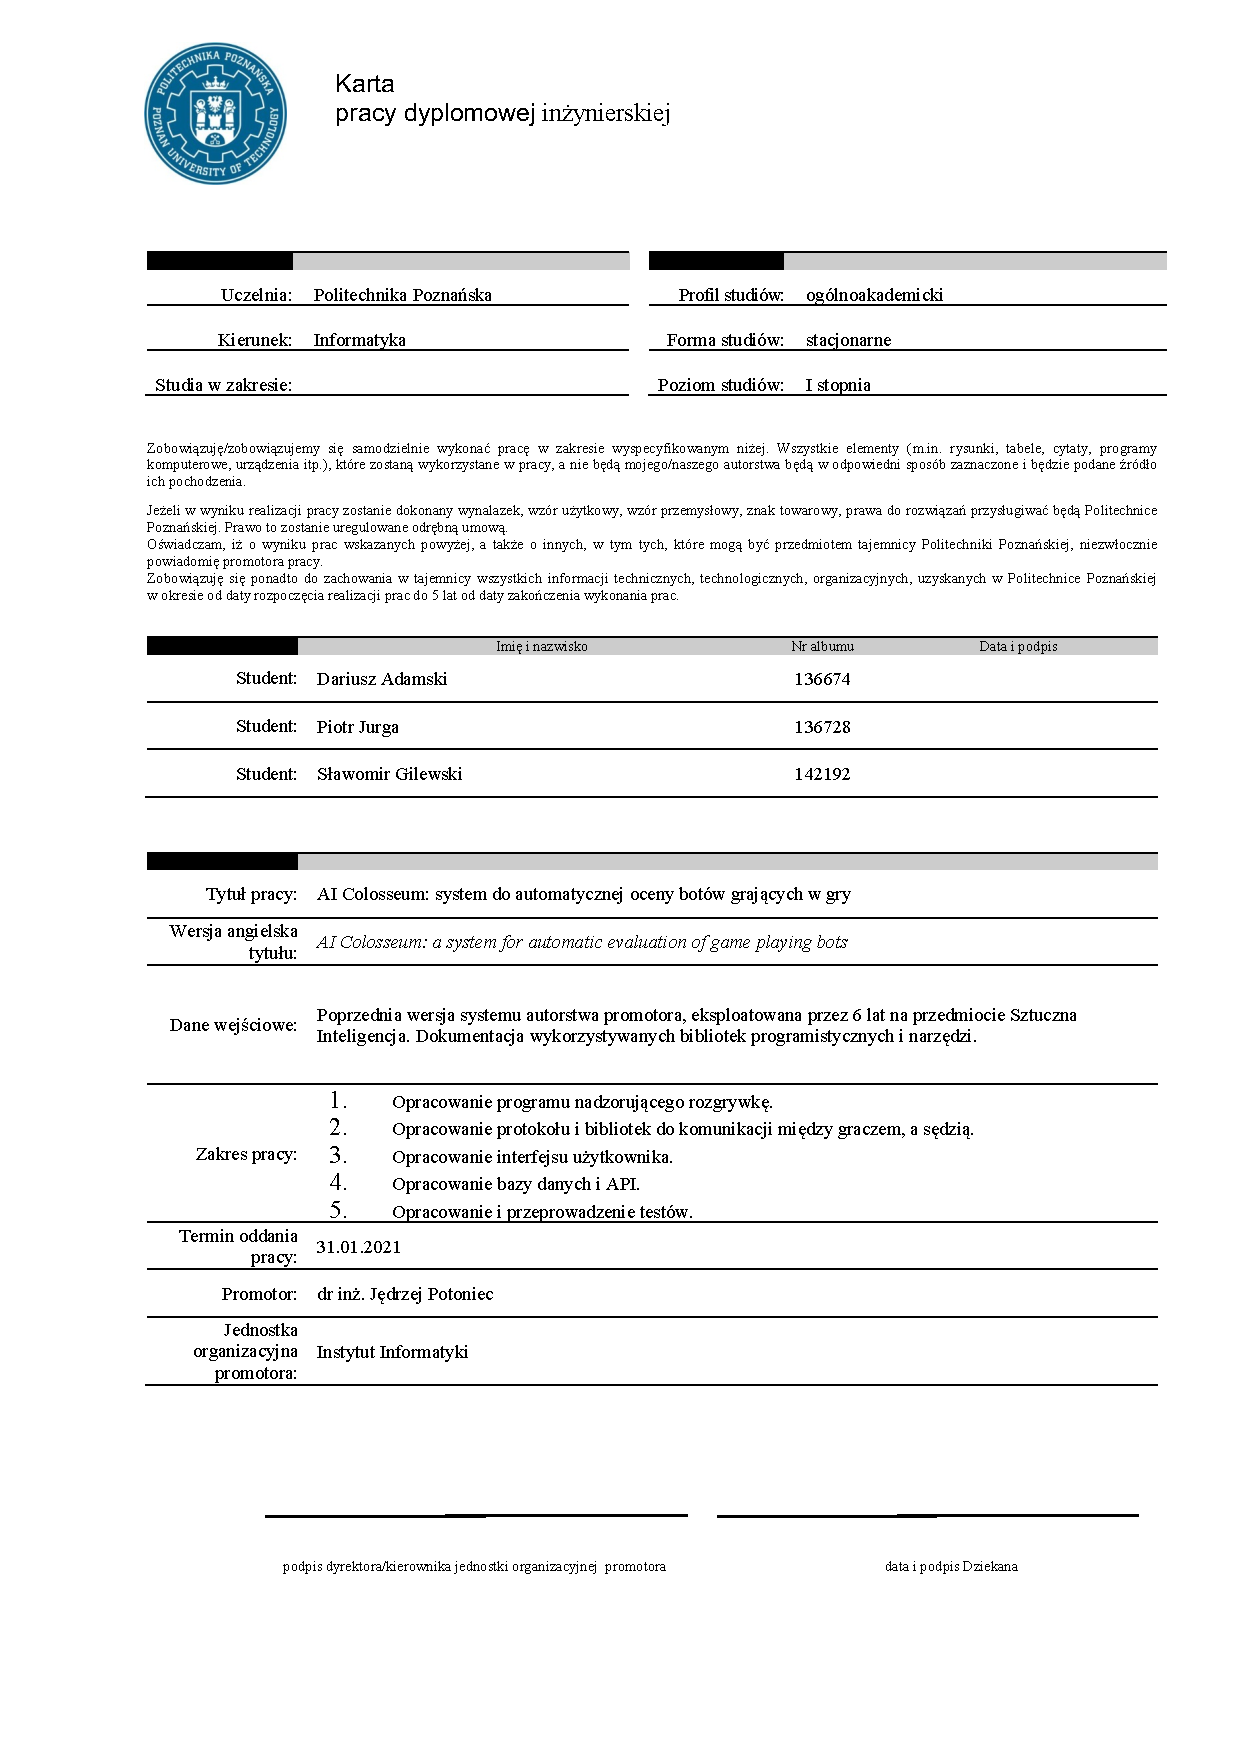
\includepdf{figures/karta_pracy.pdf}
\cleardoublepage%

%--------------------------------------
% Spis treści
%--------------------------------------

\pagenumbering{Roman}\pagestyle{ppfcmthesis}%
\tableofcontents* 
\cleardoublepage % Zaczynamy od nieparzystej strony

%--------------------------------------
% Rozdziały
%--------------------------------------

%Najwygodniej jeśli każdy rozdział znajduje się w oddzielnym pliku
\mainmatter%
\newcommand{\tw}[1]{\texttt{#1}} % tw jak TypeWriter
\newcommand{\tname}[1]{#1} % tname jak Technology Name

\chapter{Introduction} % Max
\label{chap:intro}
 
% intro to AI at PUT
% efektywny sposób nauczania
% previous attempt

In our work, we design, implement and test AI Colosseum -- an online judge system for automatic evaluation of game playing bots. AI Colosseum can, in the future, replace the current system used for the evaluation of game playing bots in the Artificial Intelligence course at the Poznan University of Technology. Our system consists of a web user interface, a database application programming interface (API) server, a compute server with a game supervisor program, and TinyBuffers -- a novel protocol and libraries for low-overhead communication between judges and players. To test AI Colosseum in practice, we implemented a judge program, reference players and game playing bots for Pentago -- a modern two-player board game. The high-level architecture of our system is shown in figure~\ref{fig:general_architecture}.

\begin{figure}[t]
    \centering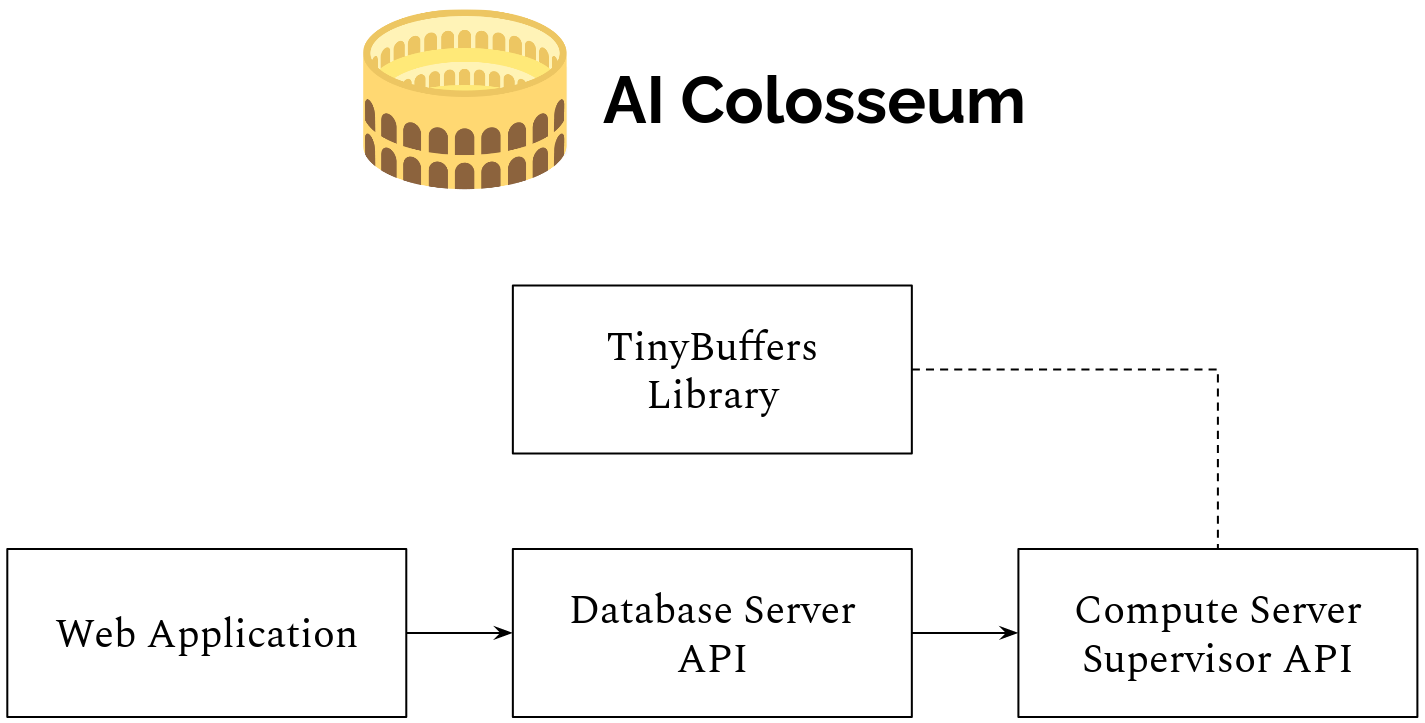
\includegraphics[width=\textwidth]{figures/arch.png}
    \caption{High-level architecture of the AI Colosseum system.}\label{fig:general_architecture}
\end{figure}

Our work is structured as follows:
In chapter~\ref{chap:background} we introduce existing online judge systems, and in detail motivate the need for a new system for automatic evaluation of game playing bots, by discussing the advantages and disadvantages of the system currently used at the AI course at the Poznan University of Technology.  
Chapter~\ref{chap:tinybuffers} specifies the TinyBuffers protocol for communication between judge and game playing bot programs. The chapter also contains a description of the TinyBuffers library implementations in the C and Python programming languages.
In chapter~\ref{chap:webapp} we describe the design and technologies of the user interface of our system. This chapter also describes the testing procedure of the application. 
Chapter~\ref{chap:database} describes the choice of the technologies used for the database API server and discusses the database schema. In this chapter, we provide a detailed description of the server  API endpoints. We also discuss the security measures implemented in the API server.
Chapter~\ref{chap:compute} describes the design and implementation of the compute servers, which orchestrate games between judges, reference players and bot submissions. First, the design of the execution environment is described. Then, the supervisor program, which also serves as a compute server, is described. Lastly, we describe the machine configuration we used for testing. Chapter~\ref{chap:pentago} contains a detailed description of Pentago -- a realistic example of a game which could be hosted on our platform. The chapter also contains a discussion of the judge program and example game playing bot implementations, benchmarks and tests.
Chapter~\ref{chap:conclusions} concludes our work and contains a discussion on possible avenues of further development of our system.

Dariusz Max Adamski designed the TinyBuffers protocol for communication between judge and game playing bots, implemented, tested and benchmarked the TinyBuffers libraries in the C and Python programming languages, created and tested the web application, created Pentago reference players in the Python programming language, drew a paper user interface prototype and designed the AI Colosseum logo. Max also helped create the compute server supervisor program and contributed to the database server API and the LXC container template. Max wrote chapters~\ref{chap:intro},~\ref{chap:tinybuffers}~and~\ref{chap:webapp} of this work.
Piotr Jurga implemented, tested and benchmarked the pentago judge and reference players in the C programming language. Piotr also created the LXC container template and set-up scripts, helped create the compute supervisor program, and contributed to the TinyBuffers design and C library. Piotr wrote chapters~\ref{chap:compute}~and~\ref{chap:pentago} of this work.
Sławomir Gilewski designed, created and tested the database server API, created the database entity-relationship diagram, relational diagram, database schema and database set-up scripts. Sławomir modified the web application and the supervisor program to connect to the database server API, and drew a user interface paper prototype. Sławomir wrote chapters~\ref{chap:intro},~\ref{chap:database}~and~\ref{chap:conclusions} of this work.
The exact contributions of each author are stored in the commit history of our project's Git repository\footnote{\url{https://github.com/maxadamski/colosseum/}}.

\chapter{Background} % Sławek
\label{chap:background}

\section{History of online judge systems}
The topic of online judge systems in education itself has been discussed for a long time, ever since 1961 when Forsythe and Wirth introduced two grading systems for the ALGOL programming language~\cite{Forsythe1965}. Educators have always seen such automatic systems as an excellent opportunity to improve the process of grading the students, as this solution introduces many possibilities and advantages. After preparing the correct environment and judges, the submitted solutions are graded automatically, which saves time for the teacher and, at the same time, allows the students to receive the feedback almost immediately. Since the ALGOL grading system, the field of online judge systems has broadened vastly. An extensive selection of those systems has been compared in ``A Survey on Online Judge Systems and Their Applications''~\cite{Wasik2017}.

Unfortunately, to our knowledge, none of the aforementioned systems is well suited for our use case. Specifically, we wanted to create a judge system, that supports turn-based board games played between bots written in different programming languages. Additionally, students writing the bots should not have to re-implement the game logic to, for example, list their valid moves. Instead, students should be able to query the judge program for information about the game state, so they can solely focus on implementing game playing algorithms. However, board games are often combinatorial~\cite{Albert2019}, so querying the judge program for a list of available valid moves is not viable without very efficient data transfer between programs written in different programming languages, especially when a game playing bot queries the judge multiple times when traversing the game state tree.

\section{Inspirations}
It is worth noting that even though our system is innovational in terms of the game mechanics, it is still an online judge system, thus allowing us to draw inspiration from some well-received systems. Both Kaggle~\cite{kaggle} and Optil.io~\cite{Wasik2016} are systems that have been functioning for years with success, and analyzing them allowed us to apply some great, working solutions to our application. Kaggle is a very popular platform mainly focused on artificial intelligence and data-mining. Even though the contest logic of Kaggle did not fit our needs, as judge programs simply compare textual file outputs, we were able to incorporate Kaggle's team mechanics into our system. Consequently, the team forming capabilities of our platform are simple but flexible, encouraging students to cooperate.

Optil.io is a platform mainly focused on optimization problems. In our opinion, the website is clear and functional, especially regarding the graphic user interface (GUI). We decided to apply a similar tab-based layout in our application, seeing how convenient it is.  We were also inspired by the user interface of Sphere~online~judge~(SPOJ)~\cite{spoj} -- a platform offering competitive programming challenges, often used to conduct didactic activities at, among others, the Poznan University of Technology.

\section{Previous system and our improvements}
Considering our system aims to replace the system which already exists and is being used every year in the Artificial Intelligence course at the Poznan University of Technology, it seemed necessary to analyze the ways in which our system improves upon the existing one.

The existing system in the AI course allows only Java as the programming language. We will go into detail about the positive qualities of this solution in chapter~\ref{chap:tinybuffers}. Still, at the very least, we are sure supporting only a single programming language is not enough. Our system introduces the ability to use a preferred programming language for writing game playing bots, starting with Python and C - which are in the top three languages in the TIOBE index~\cite{tiobe} at the time of writing. TIOBE index is an indicator informing of the popularity of programming languages, which calculation comes down to counting hits for query in search engines. On the other hand, Java, according to the TIOBE index, is losing interest: only in the year 2020, it lost almost 5\%. It is also worth mentioning, that programming language C should be known among the students, since, at the time of writing, the students should have passed ``Low-level programming in C'' after the first year of studies. We also thought about Python, because it is an easy-to-learn language, with various libraries made especially for artificial intelligence, which opens up many possibilities for the students.

A great inconvenience of the existing system was lack of any kind of administrative panel. The teacher had no means of managing the data conveniently through some sort of graphical interface. Every action or decision meant writing and executing a script and manually managing the database. Our system offers a convenient and transparent GUI, allowing both students and teachers a straightforward and comfortable way of managing their resources. More on the web application can be found in chapter~\ref{chap:webapp}.

Another shortcoming of the previous system was its database. It is a MySQL database with a hard-to-understand schema and various unnecessary leftover structures like tables and views never to be used. The communication with the database was done using PHP with many needlessly posed queries instead of one simple aggregated query. Our system introduces a thoughtfully planned PostgreSQL database, with carefully planned constraints and triggers maintaining our data integrity. We elaborate more on the database choices in chapter~\ref{chap:database}. 

\chapter{TinyBuffers}
\label{chap:tinybuffers}

\section{Motivation} % Max

% [x] Current evaluation system requires all programs to be written in Java.
% [x] Communication between JARs has minimal overhead but is inflexible.
% [x] Submitted programs in different languages require serialization because of different ABI.
% [ ] Communication by outputting single files is ill-suited for stateful tasks, such as board games, which require a judge program, which holds the game state.
% [ ] Optil.io, Kaggle, Codingame - arbitrarily structured stdin/out.
% [ ] Parsing and serializing structured text is inefficient, error-prone and not reusable across games.
% [x] Existing general data interchange formats like XML and JSON are slow.
% [x] Protocol buffers are too complex and involve code generation.
% [x] Flat buffers are simpler but still involve code generation.
% [x] Flex buffers don't have a C interface and are cumbersome compared with stdin/out.
% [x] Alternative: simple custom binary IPC protocol.

The current system for evaluating game playing bots in the AI course at PUT uses Java as the programming language for writing the judge and player programs. Using the same language simplifies communication between the programs. In Java, the player programs can communicate with the judge by directly calling methods defined by the judge program interface. After compiling the player programs, the judge program loads the resulting \tw{JAR} files and can now use the methods described by the player interface. An obvious benefit of this approach is its simplicity for the program writer, as communicating with a judge does not differ from calling methods on an object. Consequently, data serialization and file input/output are not needed for communication, which allows for minimal communication overhead. As an added plus, this approach reduces programmer errors because the Java compiler can statically verify that the programs use the defined interfaces properly.

Even though the current system possesses positive qualities, we think supporting a single programming language on a contest platform is too restrictive. Thus, we sought to support multiple languages in our system. However, communication between programs written in different programming languages introduces a problem that the current system does not have -- programs need to serialize and deserialize data when communicating because of the differences between application binary interfaces (ABI). Therefore, we needed to find a data-interchange format with minimal serialization overhead, so player programs often querying the judge for game state information, such as the available moves, do not become too slow. We considered \tname{JSON}~\cite{json} and \tname{XML}~\cite{xml}, which are human-readable text formats, but found them to be ill-suited for our task, as serialization performance was not satisfactory. We also considered binary formats, such as \tname{Protocol Buffers}~\cite{Protobuf}, \tname{FlatBuffers}~\cite{Flatbuf}, and \tname{FlexBuffers}~\cite{Flexbuf}. We rejected \tname{Protocol Buffers} because while they have better performance than human-readable text formats, they were still too slow for our use case. Additionally, both \tname{Protocol Buffers} and \tname{FlatBuffers} depend on generating serialization source code from a schema, which we decided was too complicated for the end-user. Finally, we considered \tname{FlexBuffers}, which are both fast and schema-less. However, at the time of writing, \tname{FlexBuffers} did not have an official or maintained implementation for the C language. Thus, we decided against \tname{FlexBuffers}, as supporting the C programming language was one of our main goals. 

Because we could not find a suitable data-interchange format for our system, we developed a simple binary format -- \tname{TinyBuffers}. We designed \tname{TinyBuffers} to support simple data structures, such as non-nested structures, multi-dimensional arrays and primitive types like integers and booleans. To ensure adequate performance, we designed \tname{TinyBuffers} to require minimal memory copying and allocations during serialization and data access. We describe the details of the \tname{TinyBuffers} format in the \emph{Specification} and compare its performance to implementations of some of the mentioned formats in the \emph{Benchmarks} section.

\section{Specification}

\begin{figure}[t]
    \centering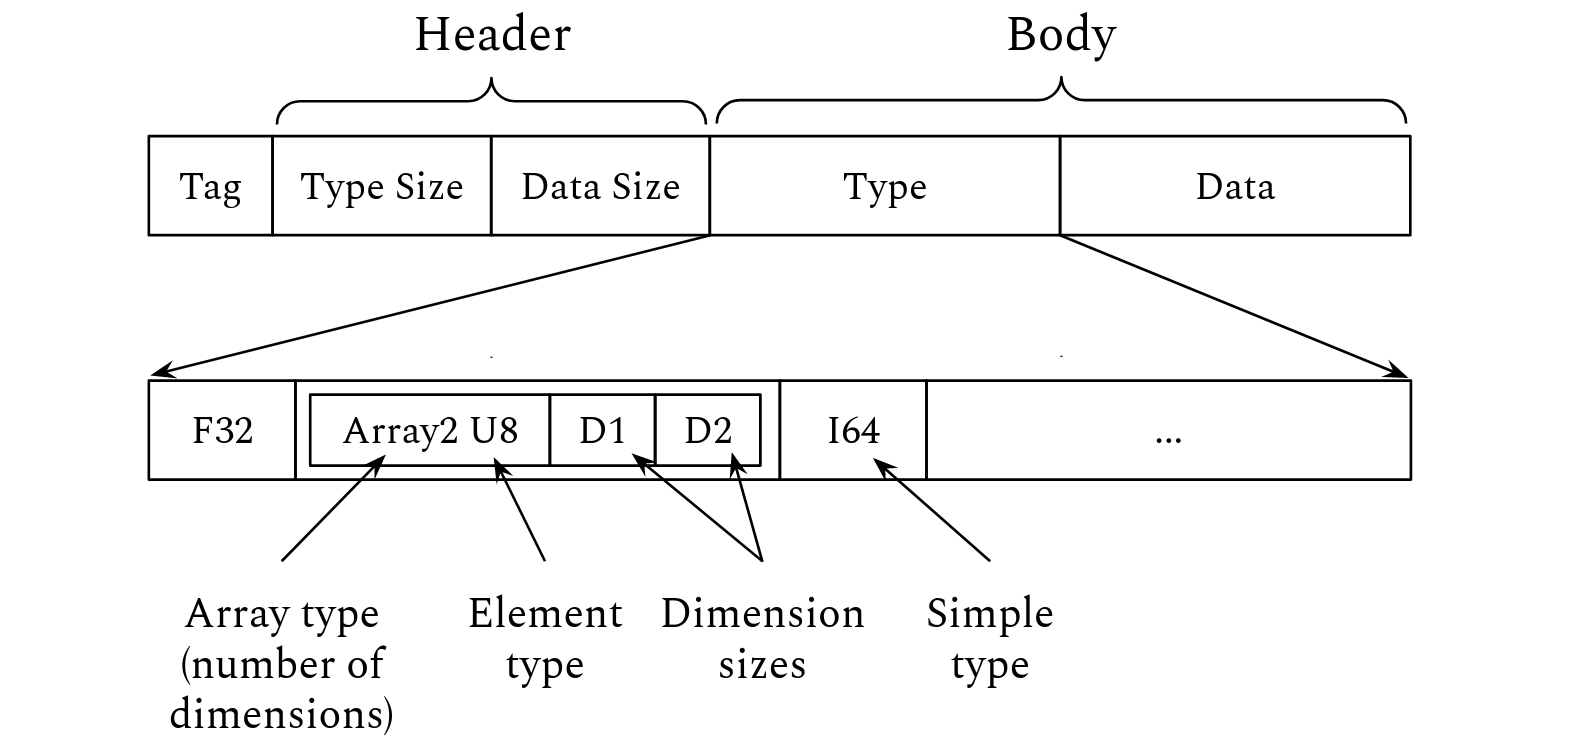
\includegraphics[width=\textwidth]{figures/tinybuffers.png}
    \caption{An example TinyBuffers packet. \tw{F32} is the 32-bit floating point type, \tw{I64} is the 64-bit signed integer type, \tw{Array2 U8 D1 D2} is the type of an array of 8-bit unsigned integers, with dimensions $D_1 \times D_2$. Refer to table \ref{tab:tinybuffers_types} for a list of all types.}\label{fig:tinybuffer_packet}
\end{figure}

A single data buffer in the \tname{TinyBuffers} binary format can be divided into three parts: the inter-process communication (IPC) \emph{tag}, buffer \emph{header} and buffer \emph{body}. The \emph{tag} field is an arbitrary 8-bit unsigned integer, that is mainly useful for implementing a jump table for reading different buffers, depending on the \emph{tag} value. The practical use of the \emph{tag} value is explained in the ``Implementations'' section. The \emph{header} can be further divided into the \emph{type size} and \emph{data size} parts, and the \emph{body} can in turn be subdivided into \emph{type} and \emph{data} parts. The \emph{type size} and \emph{data size} are simply 32-bit unsigned integers, that must be equal to the size of the \emph{type} and \emph{data} parts respectively. Taking all parts into account, the total size of a data buffer is equal to $1 + 4 + 4 + \texttt{typesize} + \texttt{datasize}$ bytes. To make understanding the format easier, an example TinyBuffer is shown in figure~\ref{fig:tinybuffer_packet}.

The \emph{body} part represents a tightly packed tuple $(x_1, x_2, ..., x_n)$, where each element is either a value of a simple type or an m-dimensional array of values of a simple type. The tuple tightly packed, because the TinyBuffers format requires, that there are no gaps of unused memory between elements of the \emph{body} buffer. The \emph{body} tuple can have no elements, in which case it is the empty tuple $()$. Of course, the size of the empty tuple is 0, as there is no data being stored.

The \emph{type} part represents the type of the \emph{body} tuple, which is the product type $T_1 \times T_2 \times ... \times T_n$. If the \emph{body} tuple is empty, then there are no types to be stored in the \emph{type} part of the buffer, so its size is 0. The type of the empty tuple is known as \tw{Unit} or \tw{Void} in some programming languages~\cite{Pierce2002}.

Moving on, a simple type is represented by a byte, where the 4 most significant bits (MSB) are all 0, and the 4 least significant bits (LSB) decide the actual type. An example simple type encoding is shown in example~\ref{ex:simple_type}. Table~\ref{tab:tinybuffers_types} lists all simple types supported by TinyBuffers and their encodings.
To construct an array type, one must first set the 4 LSB, to a simple type, which will decide the type of the array elements. Next, the second, third and fourth MSB are set to the unsigned binary number representing the number of array dimensions (with a maximum of 7 dimensions). Lastly, for each dimension, append a 32-bit unsigned integer to the type with the desired dimension size. Encoding an array type is shown in example~\ref{ex:array_type}. Computing the total size of an array value from an array type is shown in example~\ref{ex:array_size}.

\begin{table}[t]
\caption{Table of supported data types. The \emph{Type name} column shows the type notation used in our work. The \emph{C format} column shows the type name used in the format specifier of the C TinyBuffers library (syntax shown in listing \ref{lst:tinybuffers_ebnf}).}
\label{tab:tinybuffers_types}
\centering\footnotesize
\begin{tabular}{l l l c c}
\toprule
Type & Size [bits] & Type name    & C format & Type encoding\\
\midrule
Unsigned integer &  8 & \tw{U8}   & \tw{u} & \tw{0000 0000} \\
Unsigned integer & 16 & \tw{U16}  &        & \tw{0000 0001} \\
Unsigned integer & 32 & \tw{U32}  & \tw{U} & \tw{0000 0010} \\
Unsigned integer & 64 & \tw{U64}  &        & \tw{0000 0011} \\
Signed integer   &  8 & \tw{I8}   & \tw{i} & \tw{0000 0100} \\
Signed integer   & 16 & \tw{I16}  &        & \tw{0000 0101} \\
Signed integer   & 32 & \tw{I32}  & \tw{I} & \tw{0000 0110} \\
Signed integer   & 64 & \tw{I64}  &        & \tw{0000 0111} \\
Floating-point   & 32 & \tw{F32}  & \tw{f} & \tw{0000 1000} \\
Floating-point   & 64 & \tw{F64}  & \tw{F} & \tw{0000 1001} \\
Boolean          &  8 & \tw{Bool} & \tw{b} & \tw{0000 1010} \\
Character        &  8 & \tw{Char} & \tw{c} & \tw{0000 1011} \\
Array 1          & $size(T) d_1$             & \tw{T[d1]}          & & \tw{0001 TTTT} \\
Array 2          & $size(T) d_1 d_2$         & \tw{T[d1, d2]}      & & \tw{0010 TTTT} \\
Array 3          & $size(T) d_1 d_2 d_3$     & \tw{T[d1, d2, d3]}  & & \tw{0011 TTTT} \\
Array 4          & ...                       & ...                 & & \tw{0100 TTTT} \\
Array 5          & ...                       & ...                 & & \tw{0101 TTTT} \\
Array 6          & ...                       & ...                 & & \tw{0110 TTTT} \\
Array 7          & $size(T) \Pi_{i=1}^7 d_i$ & \tw{T[d1, ..., d7]} & & \tw{0111 TTTT} \\
\bottomrule
\end{tabular}
\end{table}

\begin{example}
\caption{Encoding a simple type.}
\label{ex:simple_type}
\tw{I32} is the 32-bit signed integer type, and is encoded in binary as \tw{0000 0110}.
\end{example}

\begin{example}
\caption{Encoding an array type.}
\label{ex:array_type}
\tw{U32[1024, 2024]} is a 2D array of 32-bit unsigned integers, where the first dimension has size 1024, and the second dimension size 2024. This type will be encoded as \tw{0010~0110~0x00000400~0x00000800} (dimensions written in hexadecimal for brevity). Please note, that machine words, such as dimension sizes, or multi-byte values of simple types are encoded in the little-endian byte order.
\end{example}

\begin{example}
\caption{Computing the size of an array value.}
\label{ex:array_size}
Given an array with dimensions $d_1, d_2, ..., d_n$ and element type $T$ with size $s_T$, the size of a value of this array type is $s_T \Pi_{i=1}^n d_i$.
\end{example}

Similarly to \tname{FlatBuffers}, we decided, that in the \tname{TinyBuffers} format, machine words will be stored in the little-endian byte order. Besides following FlatBuffers, we also based our decision on the fact that the most widely used processor instruction set architectures (ISA) are either little-endian or bi-endian. For example, the majority of supercomputers in the TOP500 ranking list are based on the x86\_64 architecture, which uses the little-endian byte ordering \cite{top500} \cite{top500isa}. Additionally, most desktop computers also use the little-endian x86\_64 or x86 ISAs, and more than 90\% of mobile devices use the bi-endian ARM architecture \cite{arm_investors}.

The data representation in TinyBuffers has many advantages. For example, to serialize a large array, one just needs to generate type information and copy the array data to a memory buffer without any processing (except byte swapping on big-endian architectures). Deserialization does not require any copying, as one just needs to calculate pointer offsets to tuple elements from type information. This is incredibly useful in AI Colosseum, as game playing bots will not waste any time parsing large arrays of game states while exploring the game tree, and judge programs will be able to serialize data with minimal overhead.

The TinyBuffers libraries can be optimized in the future for even better performance. For example, in programming languages, which allow for compile-time metaprogramming (like C++ templates), buffer type information could be precomputed during compilation for maximum efficiency. The same metaprogramming techniques could be used to further improve the buffer element access speed.

On the other hand, in slower dynamic programming languages like Python, TinyBuffers provide a low-friction IPC mechanism. The type information encoded in buffers can be used at runtime to access elements of an incoming TinyBuffer as if it were a plain Python object. Indeed, in the Python TinyBuffers library, we automatically convert binary arrays to Numpy arrays, to make working with data from foreign programming languages easy. Relying on Numpy also provides performance gains, as Numpy stores arrays in the exact format that TinyBuffers do, and array manipulation in Numpy is around 30 times faster than working with native Python lists \cite{Ross2014}.

\section{Implementation}

After specifying the TinyBuffers protocol, we selected named pipes as the IPC mechanism to carry the TinyBuffers. We chose named pipes because they provide a first-in-first-out (FIFO) communication channel. Other types of channels would complicate the implementation of our protocol. Additionally, named pipes provide a safe way of communication between programs in different containers. We discuss containers and the details of the bot execution environment in chapter~\ref{chap:compute}.

\subsection{C}

\begin{table}[t]
\caption{TinyBuffers C Library Functions}
\label{tab:tinybuffers_c}
\centering\footnotesize
\begin{tabular}{l l}
\toprule
Prototype & Summary \\
\midrule
\tw{i32  msendf(int f, i8 tag, char const *fmt, ...)}   & Constructs a TinyBuffer with \tw{tag} from varargs, \\
& according to a type format \tw{fmt}, then synchronously \\
& writes the buffer to descriptor \tw{f}. \\
\tw{void mscanf(u8 const *data, char const *fmt, ...)}  & Reads from a TinyBuffer \emph{data} section into varargs, \\
& according to a type format \tw{fmt} \\
\tw{i32  msend(int f, i8 tag, u8 const *buf, u32 size)} & Synchronously writes the TinyBuffer \tw{buf} with \\
& size \tw{size} and IPC tag \tw{tag}, to descriptor \tw{f}. \\
\tw{i32  mrecv(int f, i8 *tag, u8 *buf, u32 size)}      & Synchronusly reads a TinyBuffer from descriptor \tw{f}, \\
& into \tw{buf} with maximum size \tw{size} and tag \tw{tag}. \\
\bottomrule
\end{tabular}
\end{table}

The C programming language implementation of TinyBuffers exposes four main functions. Their functionality is summarized in table~\ref{tab:tinybuffers_c}.
Because the C language does not allow for type reflection, or even checking the length of variadic argument lists, we needed to specify a \tw{printf} style format language, to tell the \tw{msendf} and \tw{mscanf} how they should serialize and deserialize TinyBuffers. The resulting format language in the extended Backus-Naur form (EBNF) is shown on listing~\ref{lst:tinybuffers_ebnf}. Please refer to table~\ref{tab:tinybuffers_types} to map simple type format specifiers to types.

\newpage

\begin{lstlisting}[caption={TinyBuffers \tw{mscanf} and \tw{mprintf} format syntax in EBNF notation. Characters not recognized by the format string grammar are ignored. The percent sign is optional in the \tw{type} production rule only when using the \tw{mscanf} function}.,label={lst:tinybuffers_ebnf}]
digit     = "0" | "1" | ... | "9"
simple    = "u" | "U" | "i" | "I" | "f" | "F" | "c" | "b" 
dimension = digit {digit} | "%" ["<=" digit {digit}]
type      = ["%"] simple ["[" dimension {"," dimension} "]"]
format    = {type}
\end{lstlisting}

When sending a TinyBuffer using \tw{msendf}, for each variable in the variadic argument list, one needs to type a percent sign, followed by a simple type specifier, and optionally array dimensions separated by commas. If one wants to read an array dimension from a variable, then instead of writing a number in the dimension slot, write a percent sign and add the variable to the function argument list. An example usage of \tw{msendf} is shown on listing~\ref{lst:tinybuffers_msendf}.

\begin{lstlisting}[caption={Sending a string and a number in C.},label={lst:tinybuffers_msendf}]
char text[] = "The answer to everything";
int the_answer = 42;
msendf(fifo_out, tag, "%c[%] %u", text, strlen(text), the_answer);
\end{lstlisting}

To receive a TinyBuffer in the C programming language, first, allocate a large array of bytes, and pass it to \tw{mrecv}, to wait for an incoming TinyBuffer. After the function returns, inspect the \tw{tag} returned by argument from \tw{mrecv}. Based on the \tw{tag} and the informal contract between the judge and the bot, call \tw{mscanf} with the buffer and appropriate format string. When scanning a TinyBuffer, one may read simple types, array types and array dimensions into variables by using the percent sign and passing pointers to the given variables as variadic arguments. If one wants to ignore a buffer element, then they need to remove the percent sign before the given type. If a buffer element is ignored, the pointer to the variable is not added to the variadic argument list. Additionally, to secure oneself from a buffer overflow, one may specify an upper bound on an array dimension, using the less-than or equals operator. An example usage of \tw{mrecv} and \tw{mscanf} is shown on listing~\ref{lst:tinybuffers_mscanf}. In that example, the user checks if they received a buffer with a tag \tw{MSG\_GET\_MOVES}. Based on the judge documentation, the user knows the format of the buffer and passes it to \tw{mscanf}.

\begin{lstlisting}[caption={Receiving an array of 36 or less $6 \times 6$ Pentago boards in C},label={lst:tinybuffers_mscanf}]
u32 const max_size = 0x4000;
u8 tag, buf[max_size];
mrecv(fifo_in, &tag, &buf, max_size);
if (tag == MSG_GET_MOVES) {
    i32 boards[36][6][6];
    u32 board_count;
    mscanf(buf, "%I[%<=36,6,6]", boards, &board_count);
    ...
}
\end{lstlisting}


\newpage
\subsection{Python}

As mentioned before, the Python implementation of the TinyBuffers format benefits from the dynamic typing of the language. Listings \ref{lst:tinybuffers_mrecv_python} and \ref{lst:tinybuffers_msend_python} show examples, which are analogous to the ones shown in the previous section. However, in contrast to the previous examples, the required code is minimal as Python automatically deserializes buffers into appropriate types, based on the type information provided by the TinyBuffers format. Also notice, how the \tw{boards} object received from the \tw{col.recv} function is actually a Numpy array.

\begin{lstlisting}[caption={Receiving an array of Pentago boards in Python.},label={lst:tinybuffers_mrecv_python}]
import colosseum as col
tag, boards = col.recv(fifo_in)
print(boards.shape) # may print (32, 6, 6) 
\end{lstlisting}

Sending a TinyBuffer is almost as simple as calling a Python function. The type information is taken from the Python runtime, so the user does not need to specify it explicitly. Python integers are one exception -- because they do not have a bit-width specified, Python cannot infer whether one wants to send an 8-bit signed integer or a 32-bit unsigned integer, for example. Thus, helper functions are provided, to specify integer bit-width and sign explicitly.

\begin{lstlisting}[caption={Sending a string and a number in Python.},label={lst:tinybuffers_msend_python}]
import colosseum as col
col.send(fifo_out, tag, "The answer to everything", col.i32(42))
\end{lstlisting}

\section{Testing}

To ensure the correctness of the TinyBuffers library implementations, we created a suite of tests. Each test consisted of $n$ programs sending a specific TinyBuffer and $n$ programs receiving it, for $n = 2$ programming languages. The example programs shown in listings \ref{lst:tinybuffers_msendf}, \ref{lst:tinybuffers_mscanf}, \ref{lst:tinybuffers_mrecv_python} and \ref{lst:tinybuffers_msend_python} are actually adapted from one of our tests.

The sending and receiving programs in each test can be thought of as a complete balanced bipartite graph. In such a graph, the vertex sets $U$ and $V$ would represent our sending and receiving programs respectively, given $|U| = |V| = n$, where $n$ is the number of programming languages we supported. Thus, each test was conducted by executing all $n^2$ combinations of sending and receiving programs in different programming languages. Of course, executing the $n^2$ program combinations does not pose a large problem for modern computers. However, because for each test case we needed to write $2n$ programs, testing the TinyBuffers implementations was especially time-consuming.

We also created a series of simpler tests, that did not use the communication facilities of the TinyBuffers libraries, and only validated the content of the generated buffers. Each of these tests needed to be written $n$ times for each programming language. Given $m$ tests, we needed to execute $n \cdot m$ test programs in total.

\newpage
\section{Benchmarks}

To test the efficiency of the TinyBuffers implementations we conducted a series of benchmarks. We compared our TinyBuffers libraries with FlexBuffers. We chose FlexBuffers and not FlatBuffers or Protocol Buffers, because the latter generate code from a schema with a separate tool, and thus are not comparable to TinyBuffers, which have to generate type information during runtime. Because of FlexBuffers' poor results in Python, we also added a JSON benchmark for comparison. For the Python comparison to be fair, we used the built-in JSON library for Python benchmarks, because like our TinyBuffers implementation, it is written in Python, and not as an external C library with a Python interface.

We prepared four benchmarks in total. The first benchmark measures the time of encoding a TinyBuffer of type \tw{(U8, U32, I8, I32, F32, F64)}, the second measures the time of decoding that buffer, the third benchmark measures the time of encoding a TinyBuffer of type \tw{(U8[248,6,6])}, and the fourth benchmark measures the time of decoding that buffer. The full benchmark results are shown in table~\ref{tab:tb_bench}.

The benchmark results for the C language indicate that TinyBuffers are faster than FlexBuffers when encoding data, especially large matrices. One area where TinyBuffers are slower than FlexBuffers is reading buffers with elements of simple types only. However, please note, that FlexBuffers have the optimization advantages of the C++ language, namely compile-time computation with templates, which could have affected this benchmark. The benchmark results for Python were very surprising. The binary FlexBuffers format performed significantly worse than the human-readable JSON format, which defeats its purpose. However, at the time of writing, the FlexBuffers Python library was still in development, so performance may change in the future. Next, our TinyBuffers vastly outperformed both JSON and FlexBuffers in matrix encoding and decoding, as they were more than 100 times faster than JSON and more than 1000 times faster than FlexBuffers. Encoding and decoding simple types with TinyBuffers was slightly slower than doing so with JSON, which we expected, because the built-in Python JSON library is mature and optimized, while our library is at the proof-of-concept stage.


\begin{table}[t]
\centering\footnotesize
\caption{TinyBuffers benchmarks. The times are a sum of one million repetitions of the benchmark. All times are shown in seconds, best times are shown in bold font. Benchmarks were performed on a machine with Void~Linux, an Intel~i5~4670K~CPU, and 32GB~of~RAM. C/C++ programs were compiled with GCC and the \tw{-O3} and \tw{-march=native} optimization options.}
\label{tab:tb_bench}
\begin{tabular}{lrrcrrr}
\toprule
& \multicolumn{2}{c}{C} & \phantom{abc} & \multicolumn{3}{c}{Python} \\
\cmidrule{2-3} \cmidrule{5-7}
& TinyBuffers & FlexBuffers (C++) && TinyBuffers & FlexBuffers & JSON \\
\midrule
Encode simple & \textbf{0.0550} & 0.1788 && 3.3097 & 49.7446 & \textbf{3.1532} \\
Decode simple & 0.0433 & \textbf{0.0167} && 4.1018 & 47.8594 & \textbf{2.0930} \\
Encode matrix & \textbf{0.1675} & 0.4569 && \textbf{10.4722} & 67851.7456 & 1126.9939 \\
Decode matrix & \textbf{0.1157} & 0.1504 && \textbf{ 8.7247} & 77939.3568 &  959.4418 \\
\bottomrule
\end{tabular}
\end{table}


\chapter{Web application} % Max
\label{chap:webapp}

\section{Design process}

\begin{figure}[t]
    \centering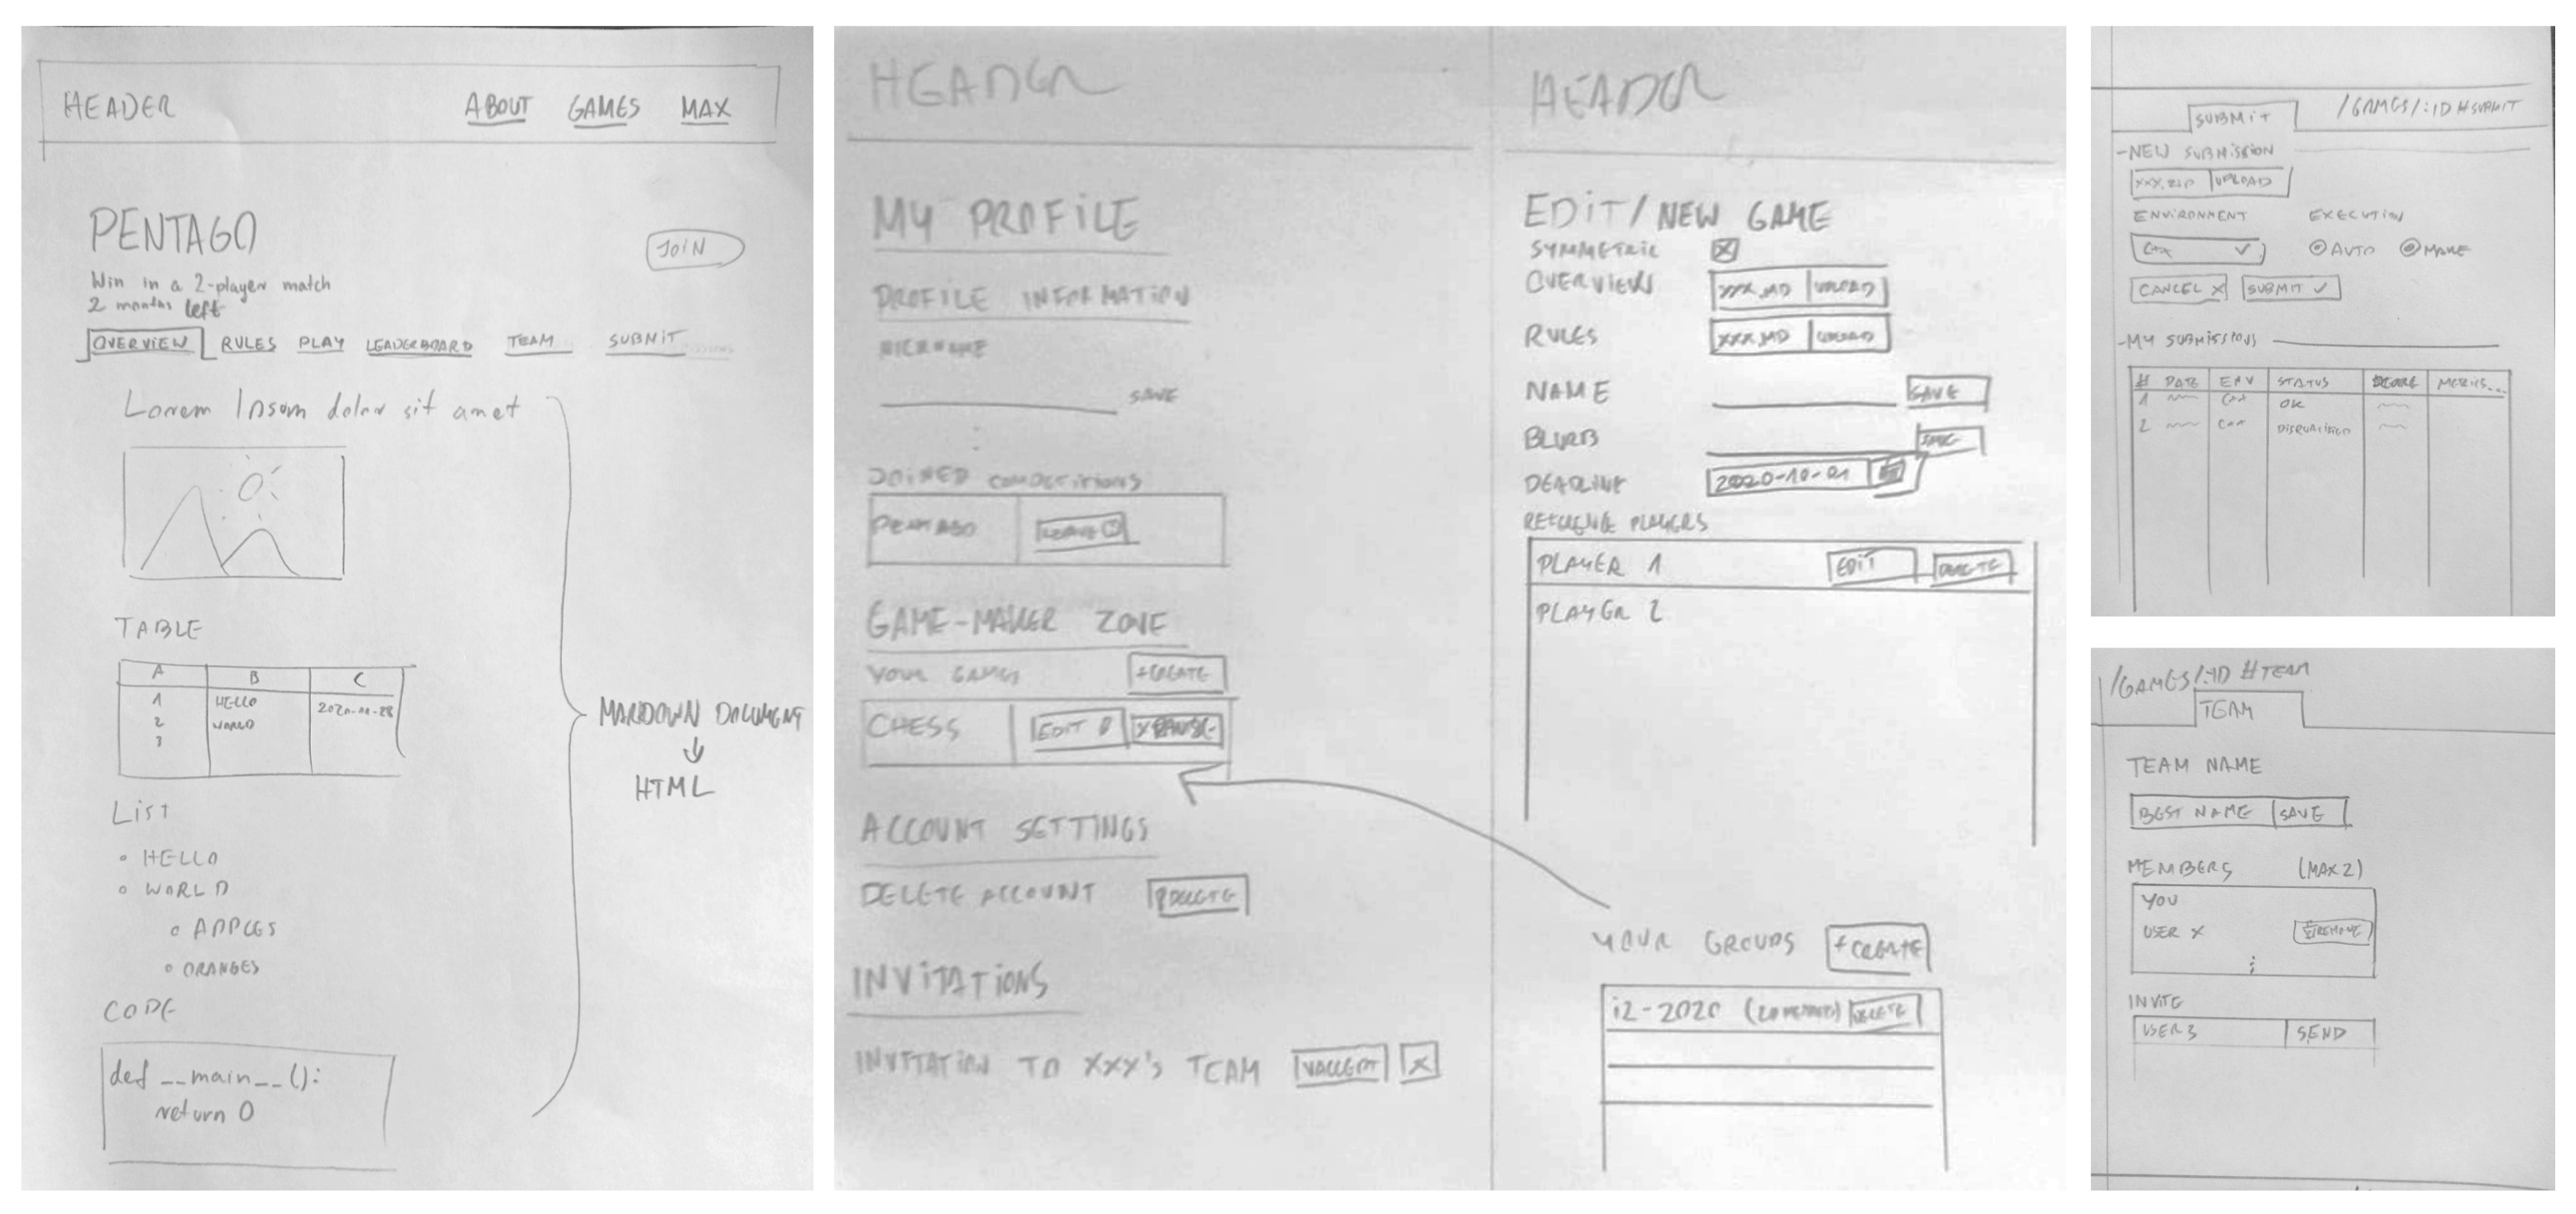
\includegraphics[width=\textwidth]{figures/proto_max.jpg}
    \caption{Selected prototypes created by Max.}\label{fig:proto1}
\end{figure}

\begin{figure}[t]
    \centering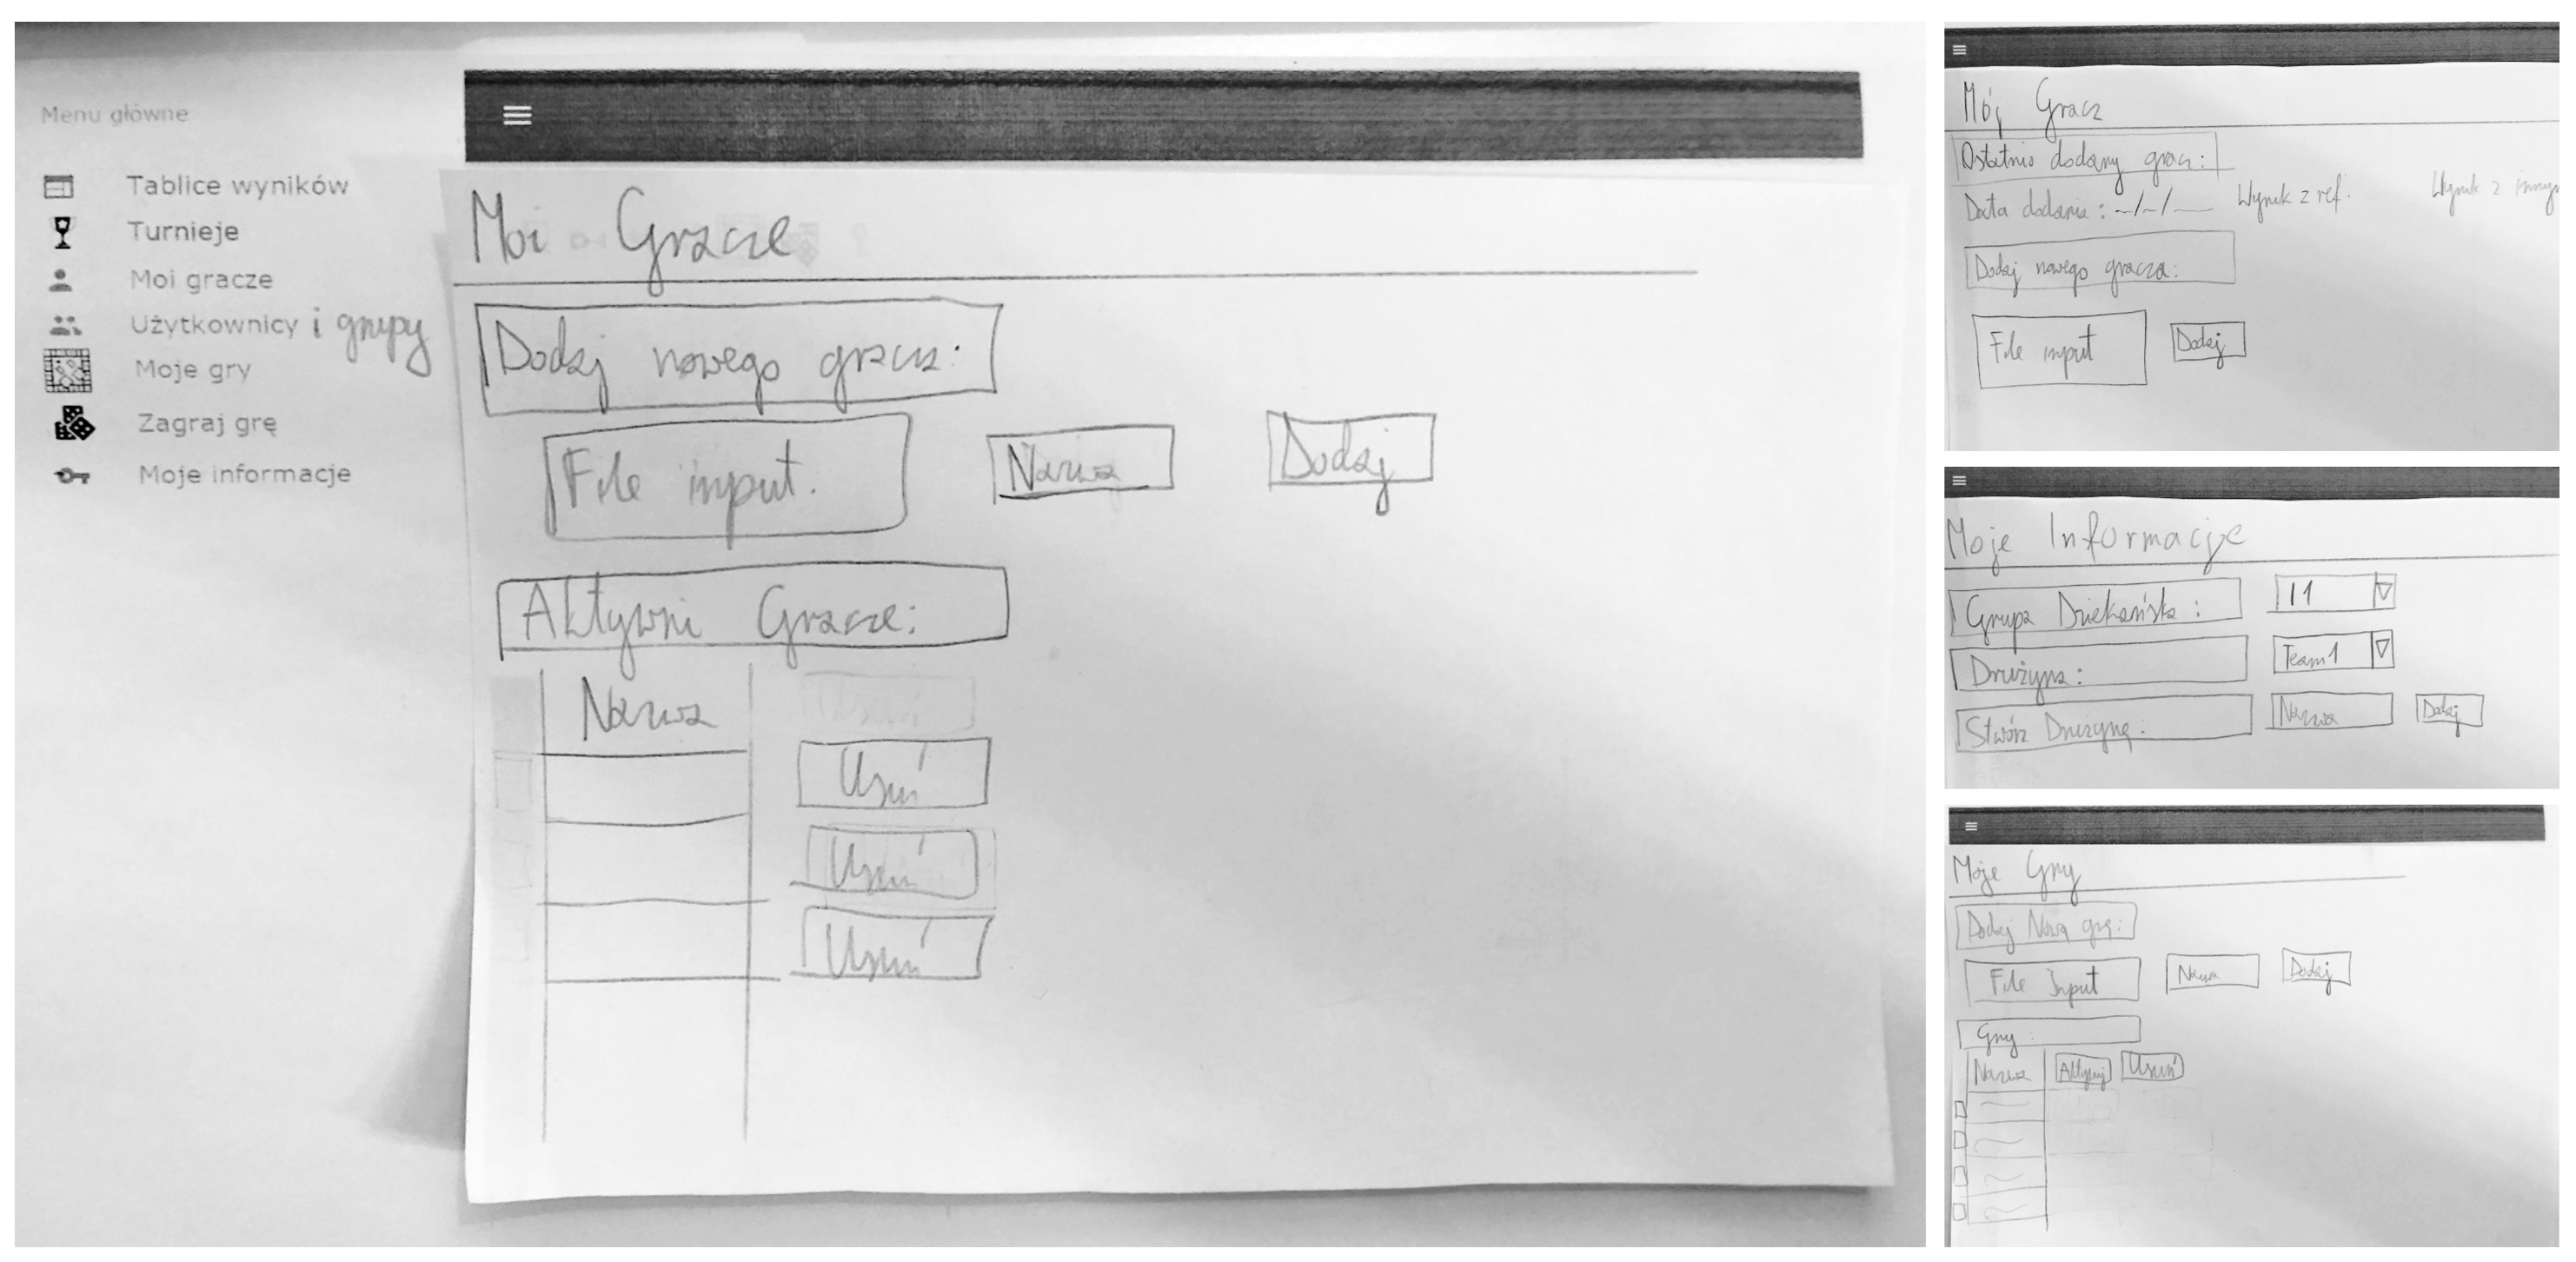
\includegraphics[width=\textwidth]{figures/proto_slawek.jpg}
	\caption{Selected prototypes created by Sławomir.}\label{fig:proto2}
\end{figure}

To create a graphical user interface (GUI) for AI Colosseum, which covers our use cases (shown in list~\ref{lst:use_cases}), is easy to use and is pleasing to the eye, we adhered to the following design strategy. Before writing any GUI code, we agreed to create paper prototypes. Each member was encouraged to research existing programming contest systems for inspiration. After preliminary research, each member, without communicating with other members, sketched a paper prototype which best fit our requirements. After everyone finished their prototypes, we presented our prototypes to each other and discussed their positive and negative aspects. We then designated one member to create a final paper prototype, which would combine the best elements of each prototype. Only after approving the final prototype did we start implementing the GUI in code. Some of our prototypes are shown in figures~\ref{fig:proto1}~and~\ref{fig:proto2}.

Because we thoroughly reviewed our prototypes, we avoided the mistake of hastily implementing a flawed or incomplete GUI design, which would lead to us wasting time redesigning the interface. Indeed, the final AI Colosseum interface did not significantly differ from the final prototype, which shows that our approach effectively limited wasted time on GUI redesigns and ensured that the interface completely covered the system's use cases.

\section{Design overview}

\begin{figure}[t]
    \centering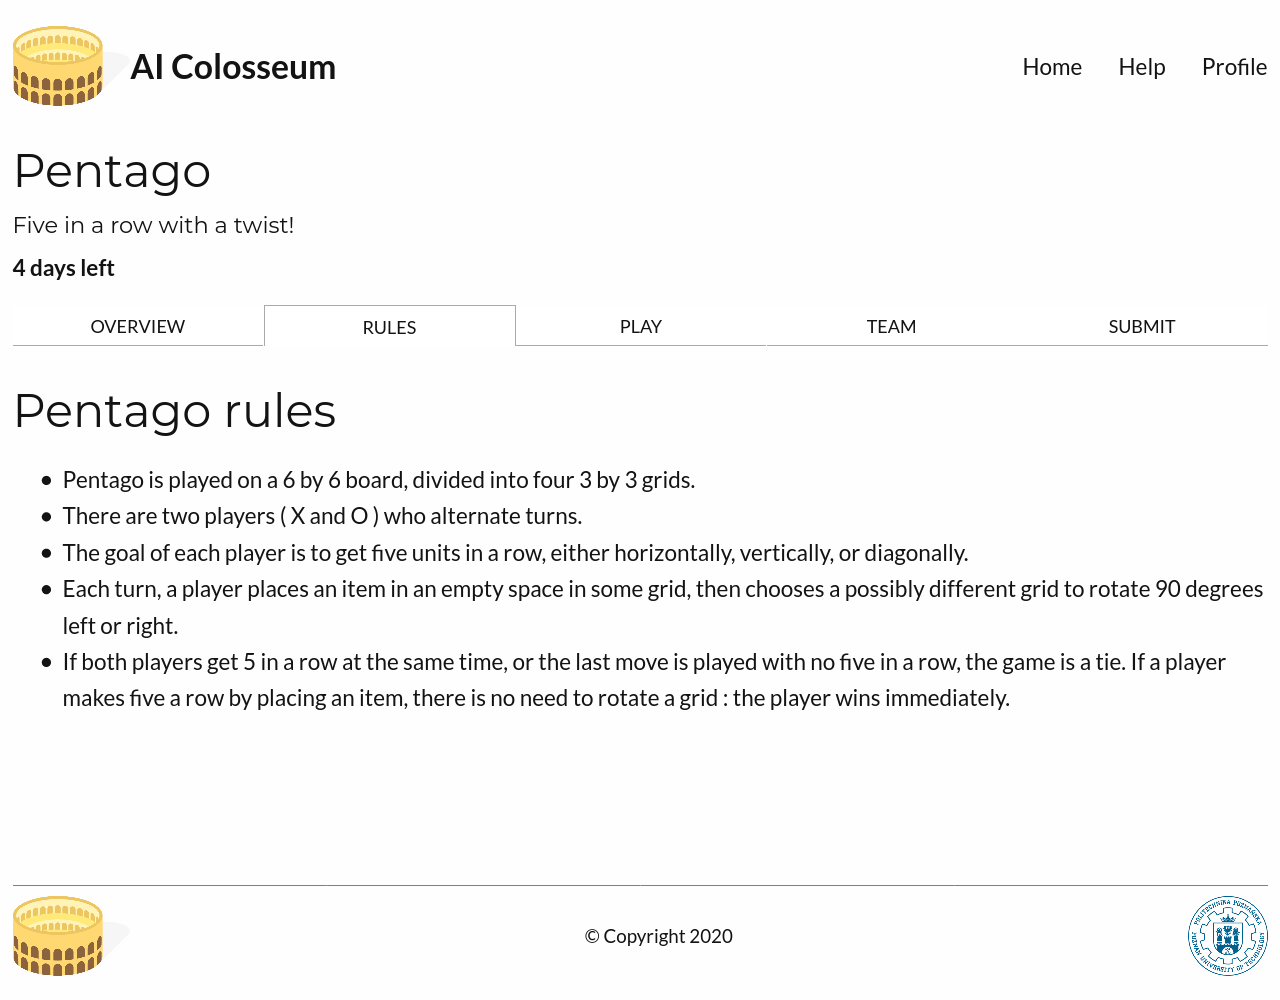
\includegraphics[width=\textwidth]{figures/www_rules.png}
	\caption{Screenshot of the AI Colosseum home page. The rules tab selected.}\label{fig:gui_home}
\end{figure}

\begin{figure}[t]
    \centering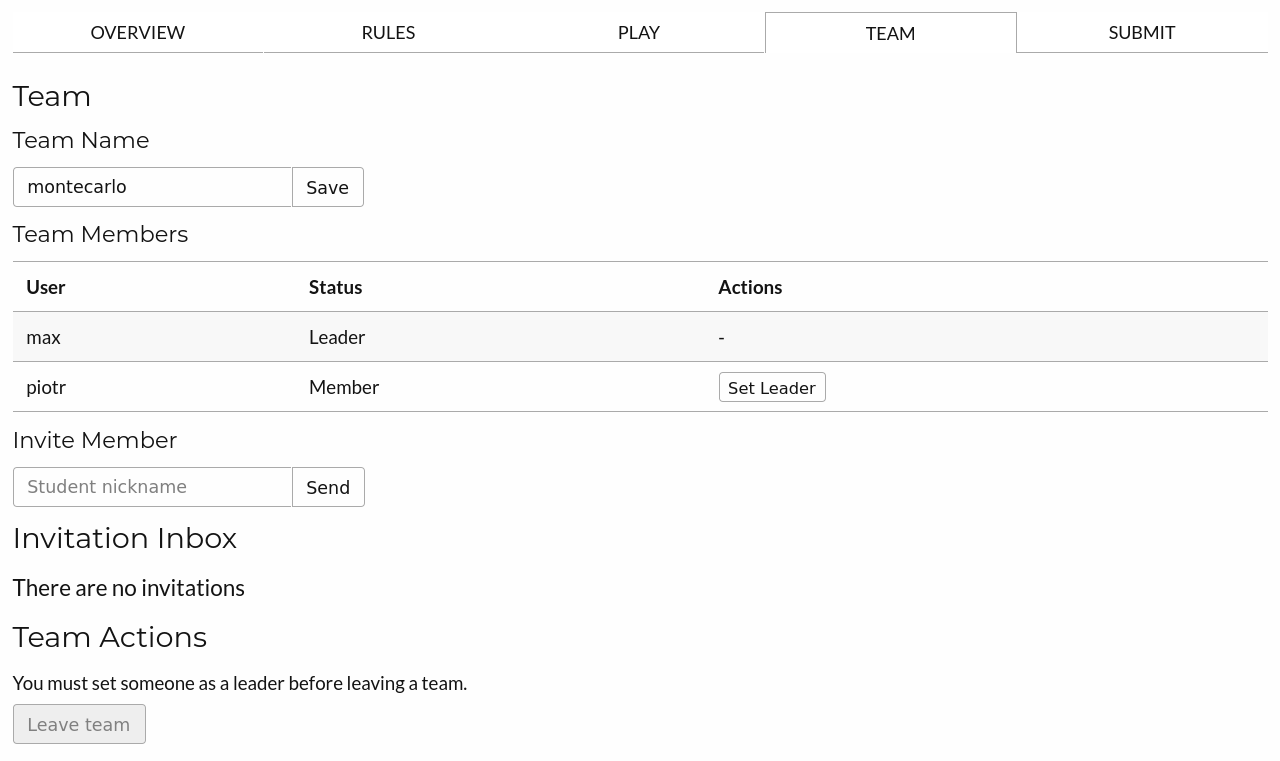
\includegraphics[width=\textwidth]{figures/www_team.png}
	\caption{Screenshot of the tome page with the team tab selected. The application header and footer are not shown.}\label{fig:gui_team}
\end{figure}

\begin{figure}[t]
    \centering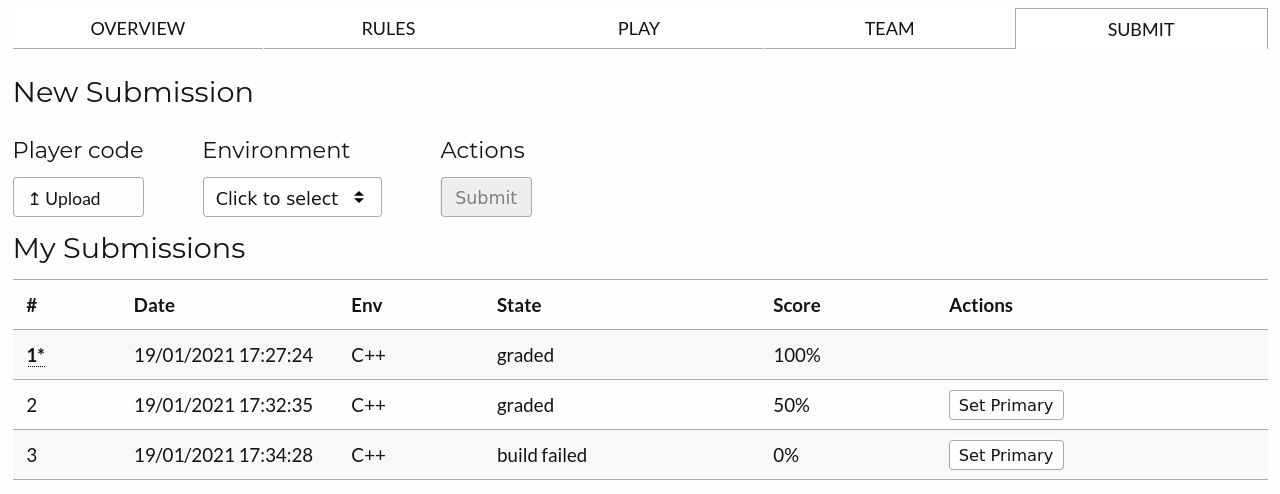
\includegraphics[width=\textwidth]{figures/www_submit.png}
	\caption{Screenshot of the home page with the submit tab selected. The application header and footer are not shown.}\label{fig:gui_submit}
\end{figure}

\begin{figure}[t]
    \centering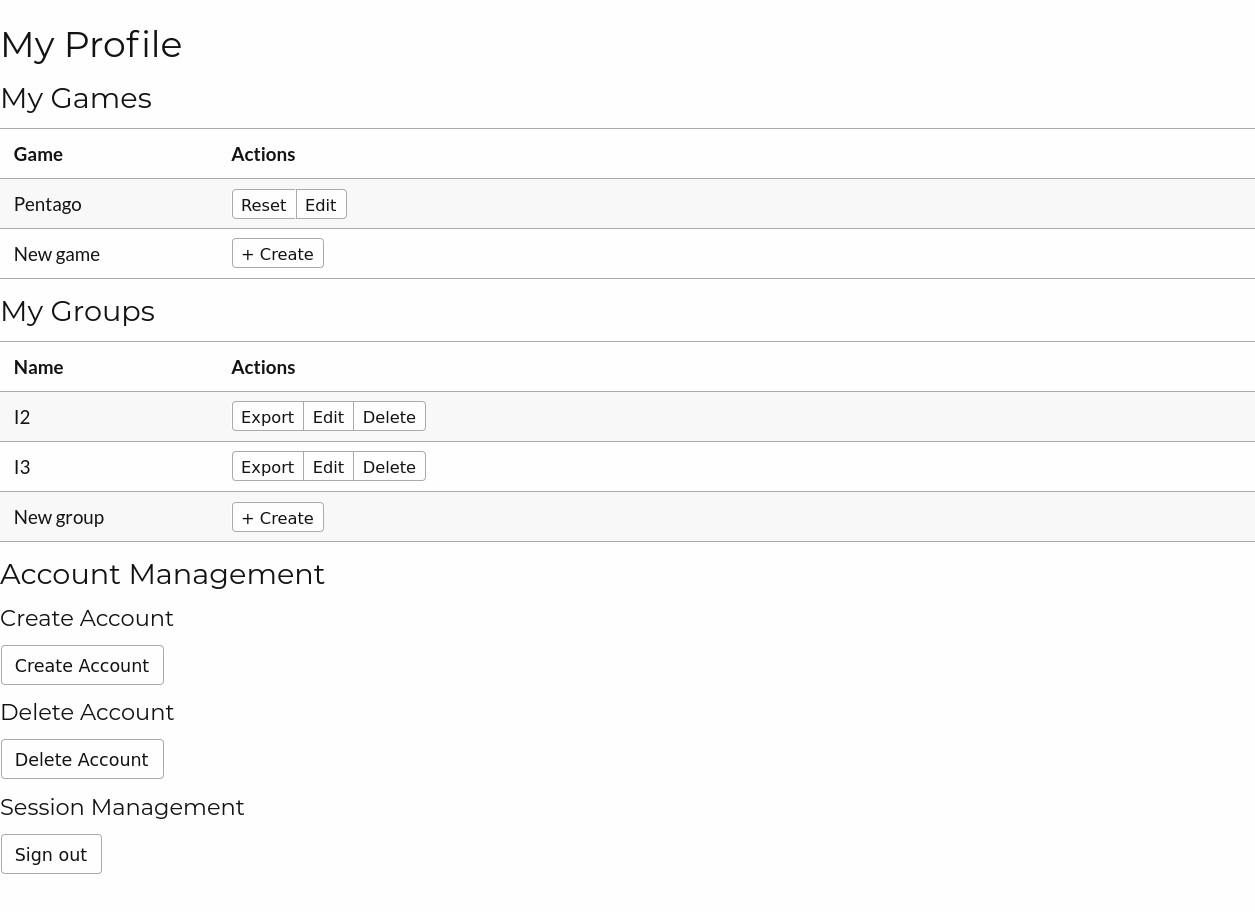
\includegraphics[width=\textwidth]{figures/www_profile.png}
	\caption{Screenshot of the teacher variant of the profile page. The application header and footer are not shown.}\label{fig:gui_profile}
\end{figure}

\begin{figure}[t]
    \centering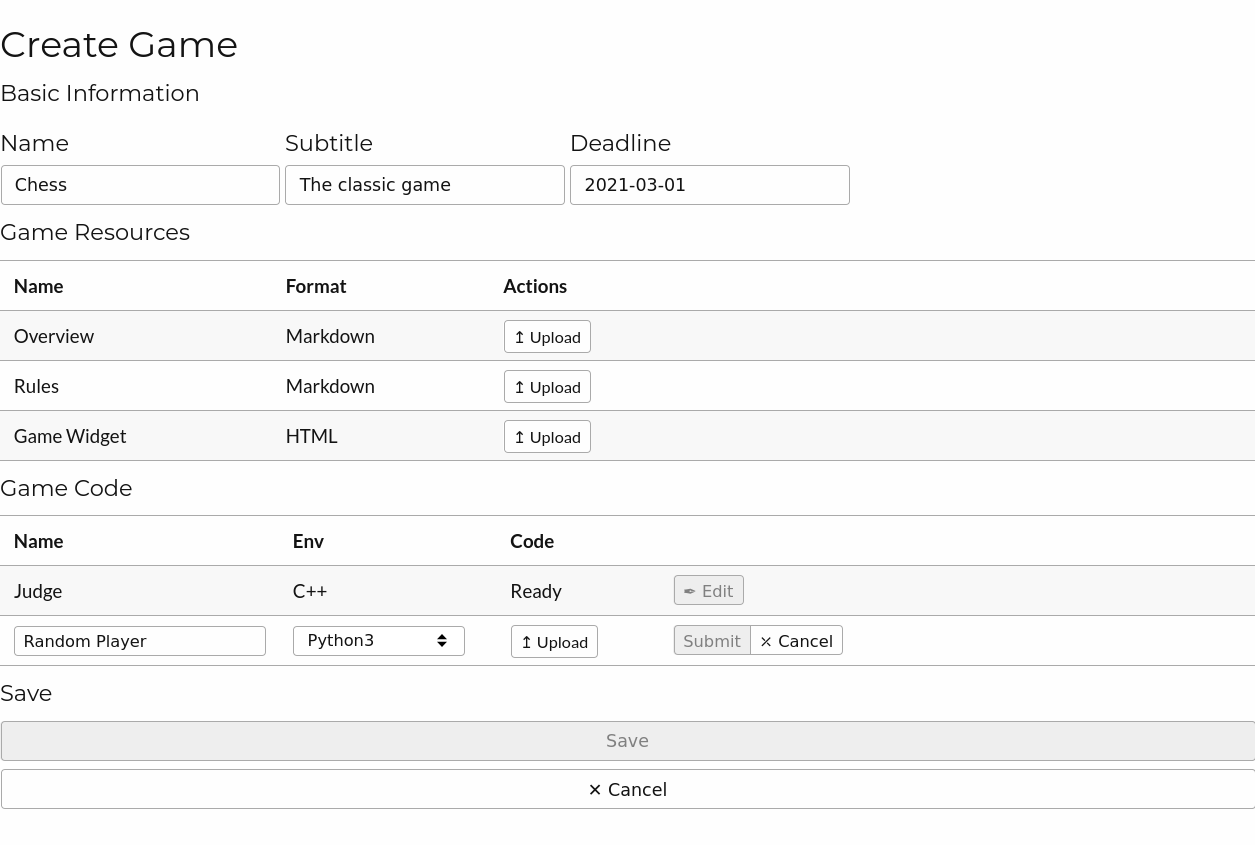
\includegraphics[width=\textwidth]{figures/www_create.png}
	\caption{Screenshot of the game editor page. The application header and footer are not shown.}\label{fig:gui_create}
\end{figure}

During prototyping, we established that we needed the following views in our application:

\begin{enumerate}
\item A view for users to familiarize themselves with a game and its rules
\item A view for users to play an interactive game
\item A view for users to manage their team
\item A view for users to submit their game playing bots
\item A view for users to sign in and manage their account
\item A view for teachers to manage student groups and games
\item A view for teachers to create and edit games
\end{enumerate}

\subsection{Home page}

As the first four views constitute the majority of user interactions in our application, we decided to merge these views into one \emph{home} page. The home page is shown upon opening our application and can be returned to by clicking the AI Colosseum logo or the \emph{home} link in the top-right corner of the application.

To avoid overloading users with information, we settled on a hierarchical tabbed home page design. For example, to see controls for submitting a game playing bot the user needs to click the \emph{submit} tab. Tabs and toolbars are common GUI elements that help organize functionality into distinct categories. An alternative approach would be to hide links to different sections of our application in an action button. We rejected that idea, as in our opinion hiding navigation options in a single button would result in a less obvious interface, and could potentially confuse users at first. Supporting our claim, a user experience study conducted by Pibernik~et~al.~\cite{Pibernik2019} found that users perceived toolbars (which are similar to our tabs) as simpler, more predictable, practical, and clearly structured than floating action buttons. Moreover, the study participants performed assigned tasks on average 2.25 seconds faster in a prototype which used toolbars instead of floating action buttons.

The \emph{overview} and \emph{rules} tab (shown in figure~\ref{fig:gui_home}) allows users to read the description of the active game and its rules respectively. After clicking on one of these tabs, a rich text document is presented. The overview and rules documents are written by the teacher in the \tname{Markdown} markup language and can contain images, tables and code excerpts, which should allow the teacher to clearly explain the game. The \tname{Markdown} documents are converted to \tname{HTML} documents after being uploaded to the database server, and when the \emph{overview} and \emph{rules} tabs are active, the \tname{HTML} document is inserted into the page code.

The \emph{play} tab allows users to interactively play the active game with a given reference player. The game interface an \emph{iframe}, which links to an \tname{HTML} document on the database server. This document is created and uploaded by the teacher and can contain arbitrary \tname{JavaScript} code to communicate with the judge over the network using \tname{HTTP} requests.

The \emph{team} tab (shown in figure~\ref{fig:gui_team}) allows users to manage their team. Regular team members can only see other team members, leave the team or accept invitations to other teams. Team leaders can additionally change the team name or invite other users to their team. Team leaders can also cancel sent invitations. We needed to create several constraints for users who wish to leave their team. Firstly, if a user is the sole member of a team, they cannot leave it. Secondly, if a team leader wants to leave their team, they must first select another member as the leader. Leaving a team will create a new team with the current user as its sole member and leader. Accepting an invitation to a team also results in the user leaving the current team. Because of that, the aforementioned constraints apply.

The \emph{submit} tab (shown in figure~\ref{fig:gui_submit}) allows users to upload their game playing bots for evaluation. To upload a bot one must click \emph{upload} and select a code file or archive, then select an execution environment and click \emph{submit}. After submitting the bot, an entry appears in the table below. The entry id, upload date, compilation status (if applicable) and bot scores are visible in each table entry. Users can refresh the application to check if the status of their submission changed. Users can also select which bot they would like to be graded in the final report by clicking the \emph{set primary} button in a table entry. A star will appear next to a table entry marked as the primary submission of their team; hovering the cursor over the star will explain its meaning.

We limit user submissions to one submission per 3 minutes per team member. The time limit can be customized in the database server configuration file. It is also worth noting that submissions belong to a team and not the user. Thus, leaving a team will cause the user to lose access to their submissions they uploaded while being a part of that team. Of course, a user can regain access to these submissions by joining the team again.

\subsection{Profile page}

The next two views are realized as the \emph{profile} page (shown in figure~\ref{fig:gui_profile}), which can be accessed by clicking the \emph{profile} or \emph{sign in} button in the top-right corner of the application. If the user is not signed in, a sign in form will be presented. After signing in, different functionality will be available at the profile page, depending on the account type.

Student accounts can change their nickname, which is shown in the team member table. Students can also change which student group they belong to.

Teacher accounts can manage student groups in the \emph{my groups} section. After clicking the \emph{create} button, a text input appears in the table. The teacher can then provide the group name and click \emph{save}. Alternatively, the teacher can click \emph{cancel}, if they do not want to create a new group after all. After creating a group, students will be able to choose it as their group. Then, at any time, the teacher can download a report for each group by clicking the \emph{export} button. The report is a table, which contains each student identifier, nickname, team name, and the score of their primary submission for the active game. The report is provided in the \tname{CSV} format, which can easily be imported into a spreadsheet application if needed.

Games saved in our system are shown in the \emph{my games} section of teacher accounts. Of course, teachers have the ability to create new games by clicking the \emph{create} button and can edit, delete or activate existing games by clicking appropriate buttons. In our project, we assumed that only one game is active at one time because at the AI course at PUT only one game is shown for the duration of one semester. Thus, activating a game results in displaying it on the home page, and blocks access to other games. Clicking the \emph{create} or \emph{edit} button loads the game editor page, which we describe in the next section. Additionally, teachers can click the \emph{reset} button to delete all student data related to a given game.

Currently, teachers can also create new teacher and student accounts by filling the \emph{create account} form in the \emph{account management} section. This functionality may be restricted in a future version of our system when we integrate Moodle account integration. We discuss potential Moodle integration in the \emph{Further work} section of our work.

Users can sign out by clicking the appropriate button in the \emph{account management} section. Students also can delete their account by clicking the \emph{delete account} button in this section. To prevent users from accidentally deleting their accounts, after clicking \emph{delete account} the user is required to type the phrase ``I want to delete my account'' and click \emph{confirm}. Alternatively, the user can click \emph{cancel} to stop the account deletion procedure.

\subsection{Game editor page}

The game editor page (shown in figure~\ref{fig:gui_create}) allows teachers to create new games or edit existing ones. To create a game, one must enter the game name, subtitle and submission deadline. The deadline field validates the input, so if an invalid date is entered, then the input is highlighted with a red wavy underline.

The \emph{game resources} table allows the teacher to upload information about the game in the form of two Markdown files and one HTML widget. We described these resources in the \emph{Home page} section.

After adding the game resources, the teacher must add entries in the \emph{game code} table. The first entry is always the judge program. The remaining entries are the reference players -- bots that each bot submitted by students will play against. To edit the judge or reference player, one must click the \emph{edit} button of the first entry. To add or edit reference players, click the \emph{create} or \emph{edit} buttons next to the given entry. When creating or editing an entry, the teacher will need to select the desired execution environment, upload the program code and click save. If the environment was not selected, or program code of an entry was not uploaded, the \emph{save} button for the entry will be disabled. Editing or adding an entry can be cancelled by clicking the \emph{cancel} button. Doing so will revert any changes made to an entry.

After the game form is completed, click \emph{save} to submit the game. Alternatively, click \emph{cancel} to discard the form.

When editing an active game, the teacher will only be able to update the code of the reference players. We decided, that removing and adding reference players should not be possible, because changing the number of reference players in the middle of a competition could potentially invalidate the scoring of existing user submissions. For example, removing the only reference player would result in every student submission having a 0\% score. Therefore, we decided, that to change the game code or add reference players, one has to create a new game. Besides the mentioned constraint, teachers are free to modify game resources, code and metadata as they wish.

Also, please note, that besides client-side validation, all inputs are validated by the database server. Please refer to chapter~\ref{chap:database} for more information on data validation.


\section{Technologies}

% TODO(max) how exactly Reactive programming helps
% TODO(max) discuss accessibility (semantic HTML5 tags)

For our project, the GUI needed to be as widely accessible as possible. Therefore, we decided against using platform-specific or proprietary application development frameworks such as \tname{Cocoa} for \tname{macOS} or \tname{Windows Forms}. Of course, while the primary user platform we targeted in our project was desktop computers, we also wanted to enable mobile and tablet device users to use the AI Colosseum system. Thus, we excluded strictly desktop or mobile application frameworks like \tname{GTK+}, \tname{Qt}, and \tname{Android}, as using them would limit the user to one type of platform. Taking that into account, building a web application turned out to be the most accessible solution. Consequently, anyone using a modern web browser can utilize the full functionality of the AI Colosseum system.

After we decided to develop a web application, we faced the dilemma of choosing between creating a single-page application (SPA) or a multi-page application. A single-page web application loads its resources once from the server. After initialization, website content is rewritten with client-side JavaScript code~\cite{Flanagan2014SinglePageApp}. Further communication with the application server is done on-demand by sending asynchronous JavaScript and XML (AJAX) requests, which do not require reloading the page. Although fetching one large bundle of code upon entering a website may be slower than loading medium-sized bundles of code every time a user navigates to another page, in our opinion, it ultimately provides a more native user experience, because users of our system do not have to wait for the website to reload after sending a form or navigating to a different page. Another benefit of this approach is that the database server does not have to concern itself with generating \tname{HTML} documents. This lowers the CPU load of the server and increases response time.

As the backbone of our web application, we chose \tname{Vue.js}~\cite{vuejs} -- a popular, relatively small (33KB compressed) JavaScript framework used for creating single-page applications. \tname{Vue.js} uses reactive programming for defining user interfaces. Reactive programming is a declarative programming paradigm, which automates data flow in a stateful program. Consequently, we did not have to manually update or redraw application content on each state change, as reactive variables observe their dependencies, and recompute their values automatically when any of them change. We also use the Vue-Router plugin for \tname{Vue.js}, which automatically manages transitions between pages of our application.

While developing the web application, we limited the use of external libraries, relying on standard browser APIs where viable. There were two instances of this approach, which significantly reduced the size of our application. Firstly, instead of using a popular HTTP request library like \tname{Axios}~\cite{axios}, we used the standard \tw{fetch} API~\cite{mozilla_fetch} to perform asynchronous HTTP requests. Secondly, instead of managing application state with a library like \tname{Vuex}~\cite{vuex}, we created a reactive state dictionary using the \tw{defineReactive} function provided by \tname{Vue.js}, and used the \tw{localStorage}~\cite{mozilla_fetch} browser API for storing user data. According to \url{packagephobia.com}, at the time of writing, adding the \tname{Axios} library would increase the published application size by 363KB, and adding the \tname{Vuex} library would add additional 357KB.  As our application size was 327KB in total, these two packages would triple its size (all sizes before compression). The increased size would make loading the application much slower on slow internet connections or older devices. Thankfully, the web browser APIs and Vue alone provided all the functionality we needed.

Instead of writing plain \tname{HTML} and \tname{CSS} code, we opted to use \tname{Pug.js}~\cite{pugjs} and \tname{Stylus}~\cite{stylus}, which are alternative syntaxes for these languages. Both languages adhere to the off-side rule, which delimits blocks of code by indentation. Choosing \tname{Pug.js} and \tname{Stylus} was mostly a subjective choice, as we prefer indentation-sensitive languages. However, there are additional advantages to using these languages. In particular, \tname{Stylus} supports user-defined mixins, which allowed us to reduce style code duplication. Mixins are similar to the \tw{\#include} preprocessor directive in the C programming language; invoking a mixin in a style class includes the mixin's contents~\cite{stylus_mixins}. We created parametric mixins that act as shorthand for specifying commonly co-occurring \tname{CSS} properties. \tname{Stylus} also supports compile-time code generation. For example, we used these code-generation capabilities for generating multiple reusable classes with \tw{margin} and \tw{padding} properties sized according to our chosen spacing scale.

All \tname{Vue.js}, \tname{Pug.js}, \tname{Stylus}, and image files used in our application are preprocessed, transpiled, minified, compressed, and bundled together using the \tname{Parcel}~\cite{parcel} bundler. We specifically used \tname{Parcel}, because it does not require any configuration. Before discovering \tname{Parcel}, we considered using Webpack as the bundler for our project. However, its configuration is so complex that we could not configure it to work with our chosen technologies. Additionally, \tname{Parcel} is up to 20 faster than Webpack and alternative bundlers, because of multi-core compilation and caching. \tname{Parcel} also supports live code reloading, which allowed us to immediately see the changes in our application as we edited its source code. This improved development speed and comfort.

Another feature of \tname{Parcel} we used was code splitting -- the ability to load JavaScript modules lazily. We used code splitting to combine the benefits of single-page and multi-page applications. Instead of loading the entire application code at the start of the application, the page code is fetched on-demand. This approach should not be confused with requesting dynamic content in a multi-page application. The chunks of code created by \tname{Parcel} are static -- they do not depend on the application state, and the server does not have to dynamically generate any \tname{HTML}.

Similar to other AI Colosseum modules, we managed the development environment with Anaconda~\cite{anaconda}. Upon creating the virtual environment, Anaconda installs \tname{Node.js}~\cite{nodejs} -- the JavaScript runtime, and \tname{Yarn}~\cite{yarn} -- a \tname{Node.js} package manager. After \tname{Node.js} is installed on the system, \tname{Yarn} downloads all required JavaScript packages. Afterwards, \tname{Parcel} outputs static \tname{HTML}, \tname{CSS}, and JavaScript files, which can be placed on any hosting service like Github Pages, or served from a web server like \tname{Nginx}~\cite{nginx} or the \tname{Apache HTTP server}~\cite{apache}. Finally, an \tname{HTTPS} certificate must be set-up because we designed the database API server to require a secure \tname{HTTPS} connection. 

\section{Quality assessment}

\begin{figure}[t]
    \centering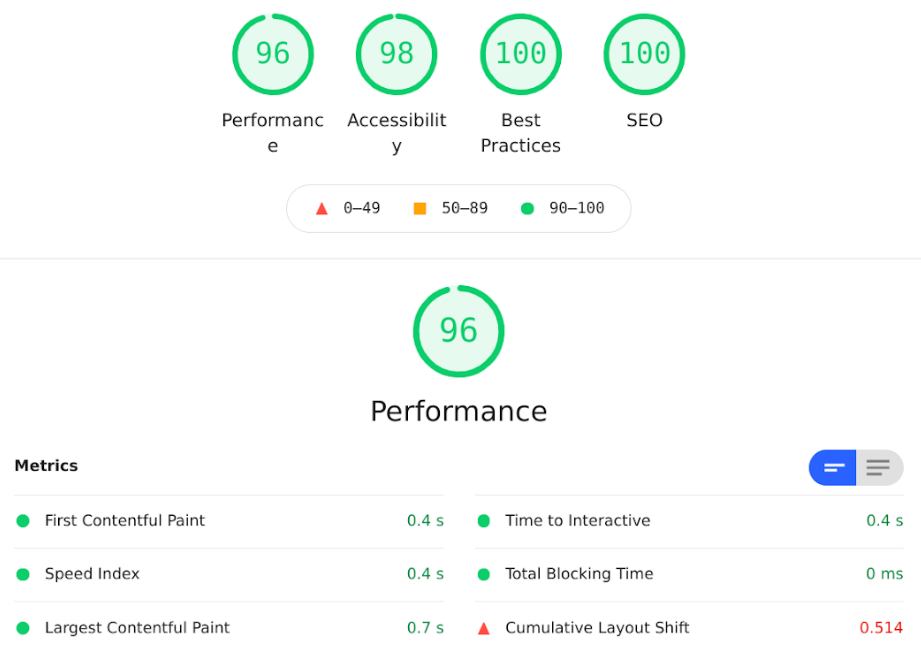
\includegraphics[scale=0.35]{figures/lighthouse.png}
	\caption{Summary of the Google Chrome Lighthouse report for our web application.}\label{fig:lighthouse}
\end{figure}

We assessed the completeness of the web application by manually testing each use case of the teacher, student and team leader roles (shown in list~\ref{lst:use_cases}). For each use case, we also tried intentionally inputting invalid data where possible, to check if our application reacts appropriately by showing an error message and rejecting the malformed input. After verifying that every use case is covered by our web application, we concluded that the functionality of the application is complete.

\begin{mylist}
\caption{Teacher, student and team leader use cases.}
\label{lst:use_cases}
\begin{itemize}
\item Teacher:
    \begin{itemize}
    \item Activates, adds, edits, deletes a game
    \item Adds, renames or deletes a student group
    \item Downloads a report of a student group
    \end{itemize}
    
\item Student:
    \begin{itemize}
    \item Reads the game description and rules
    \item Plays an interactive game
    \item Submits a game playing bot for evaluation
    \item Accepts an invitation to a team 
    \item Changes their nickname
    \end{itemize}

\item Team leader:
    \begin{itemize}
    \item Changes team name or leader
    \item Sends invitation to a team
    \end{itemize}
\end{itemize}
\end{mylist}

Next, we used Google Chrome Lighthouse~\cite{Lighthouse}, which is an automated webpage quality testing tool built into the Google Chrome browser, to measure the application performance, accessibility and best practices. Our application has achieved very high scores in the Lighthouse audit, with 96 out 100 points in performance, 98 points in accessibility, 100 points in best practices and 100 points in search engine optimization (SEO). One of the concrete metrics Lighthouse uses for scoring is time until a website becomes fully interactive (TTI). According to the Lighthouse report, our application becomes fully interactive in just 0.4 seconds. For comparison, \tname{Optil.io}, a website with similar functionality achieves 81 out of 100 points in performance and becomes fully interactive in 1.5 seconds. While our application has 3 times lower TTI, we note that both websites have high performance, because according to the Lighthouse metrics, a website is slow, when it becomes fully interactive after 7.3 seconds or more. The summary of the Lighthouse report for our application is shown in figure~\ref{fig:lighthouse}. The full description of the Lighthouse audits and metrics is available at the Google Lighthouse performance audit website~\cite{lighthouse_metrics}.

\chapter{Database server}
\label{chap:database}

\section{Database} %Sławek
\subsection{Choice of the database management system}
To choose the ideal database management system for our project, we had to study each possibility along with its capabilities and limitations.  Understanding the primary purpose, requirements we will go through below, and how we want to use and access our data was crucial before making the decision. With many different systems to choose from and most of them widely used in various flag companies, the choice could seem insignificant, however, choosing the wrong solution might have come as an obstacle in the future, as the project grows and the problem becomes difficult to overcome.

The first and obvious decision to be made was whether our database model should be relational or not. We decided to build a relational SQL database for a number of reasons. Since the beginning, our project's purpose suggested that the data stored will be highly structured, with several objects linked to one another, for instance, every user was to be associated with a team, with each team linked to multiple submissions. For the potential application owner, it was essential to have a basic understanding of how the data was structured, which is very clear in the case of relational databases. It was also imperative that the transactions made were atomic -- the situation where the student submitted an incomplete solution for evaluation was unacceptable. Since our system was supposed to be fail-safe, we also had to ensure that post-transaction changes written to disk are persistent even if a system failure occurs. Once the user made the changes in the application, they had to be absolute. Both of the mentioned features suggest that the chosen system had to provide atomicity, consistency, isolation and durability (ACID) properties, which is only possible in relational databases. We considered the non-relational solution but found it unfit for our project, due to lack of ACID support. Another disadvantage was that the NoSQL databases are relatively new compared to classic relational ones, which means they may be less stable and solving the problems may prove to be more time-consuming.

Once we have decided on the database model, we had to pick a suitable database management system. We considered three, most reliable and popular relational database management systems: MySQL~\cite{mysql}, MariaDB~\cite{mariadb} and PostgreSQL~\cite{postgresql}. Initially, we focused on choosing between the first two, but in the end, Postgres turned out to be a better choice.

First of all, it is essential to mention that since Oracle acquired MySql with unclear intentions, the open-source nature of MySQL became uncertain, which already made us sceptical of using it. In comparison, MariaDB was made by the original developers of MySQL and is guaranteed to stay open source -- all code in MariaDB is released under General Public License (GPL) and Lesser General Public License (LGPL). Some parts of the MariaDB code are public domain or released under Berkeley Software Distribution License (BSD), which has minimal restrictions on the use and distribution of the software it covers. Even though MariaDB is relatively new, it has made numerous changes that positively affect its performance. Complete list of the changes can be found on the MariaDB Foundation's website, though the most significant was replacing MyISAM and InnoDB engines with Aria and XtraDB, which are much faster especially at the GROUP BY level. It seemed that the MariaDB would be a perfect choice, being better than MySQL in every aspect, but PostgreSQL turned out to be even better in several aspects. 

Postgres has shown even better overall performance than MariaDB. It also has many features that the latter does not, such as Materialized Views, Partial Indexes, Range Types and User-Defined Types which may prove useful in optimizing the database performance even further. We also found that the procedural language PL/PgSQL and its trigger syntax is more intuitive than MySQL's procedural language. Thus, the database management system we ultimately decided on was relational PostgreSQL.

\subsection{Database overview}


Considering the database is the backbone of our system, we had to think carefully about its contents and structure. We had to thoroughly go through not only our current expectations but also the future work possibilities. Even though at the time of our work, we only considered one active game at the time, this might change in the future, and it was our responsibility to make sure, that these changes can and will be as seamless as possible. 

Our project offers its services to two different types of users: students and teachers, each of them with different purpose and permissions. Each student has to be present in two groups: student group, which mirrors the groups present at the university and student team, in which students work together on their solutions. Every team member can upload his solutions, but only the leader can manage the team name and members. In general, the objects we store in our database are games and bots (submissions) associated with those games, together with all the necessary information. Every game has its own set of reference submissions, uploaded by the teachers, but only one game at the time can be active. Both games and submissions can be written in any programming language (environment) supported by our system. 

Each semester, the teacher can activate one of the mentioned games for the students to compete in. After the semester ends all the previous semester information becomes redundant for the teacher, therefore once a new game is activated, all the previous semester's data about students and their submissions are reset. However, the chosen design of the database makes it simple to extend, so that in the future, the team can have separate submissions for different games. 

It is also necessary to mention that there are two types of outcome depending on the bots taking part in the game: tournament result -- between two bots submitted by the different student teams and reference result -- between student's bot and the reference bot. Taking all of the mentioned requirements into consideration, we created a conceptual model in the form of an entity-relationship diagram shown in figure~\ref{fig:er_diagram}

\begin{figure}[t]
    \centering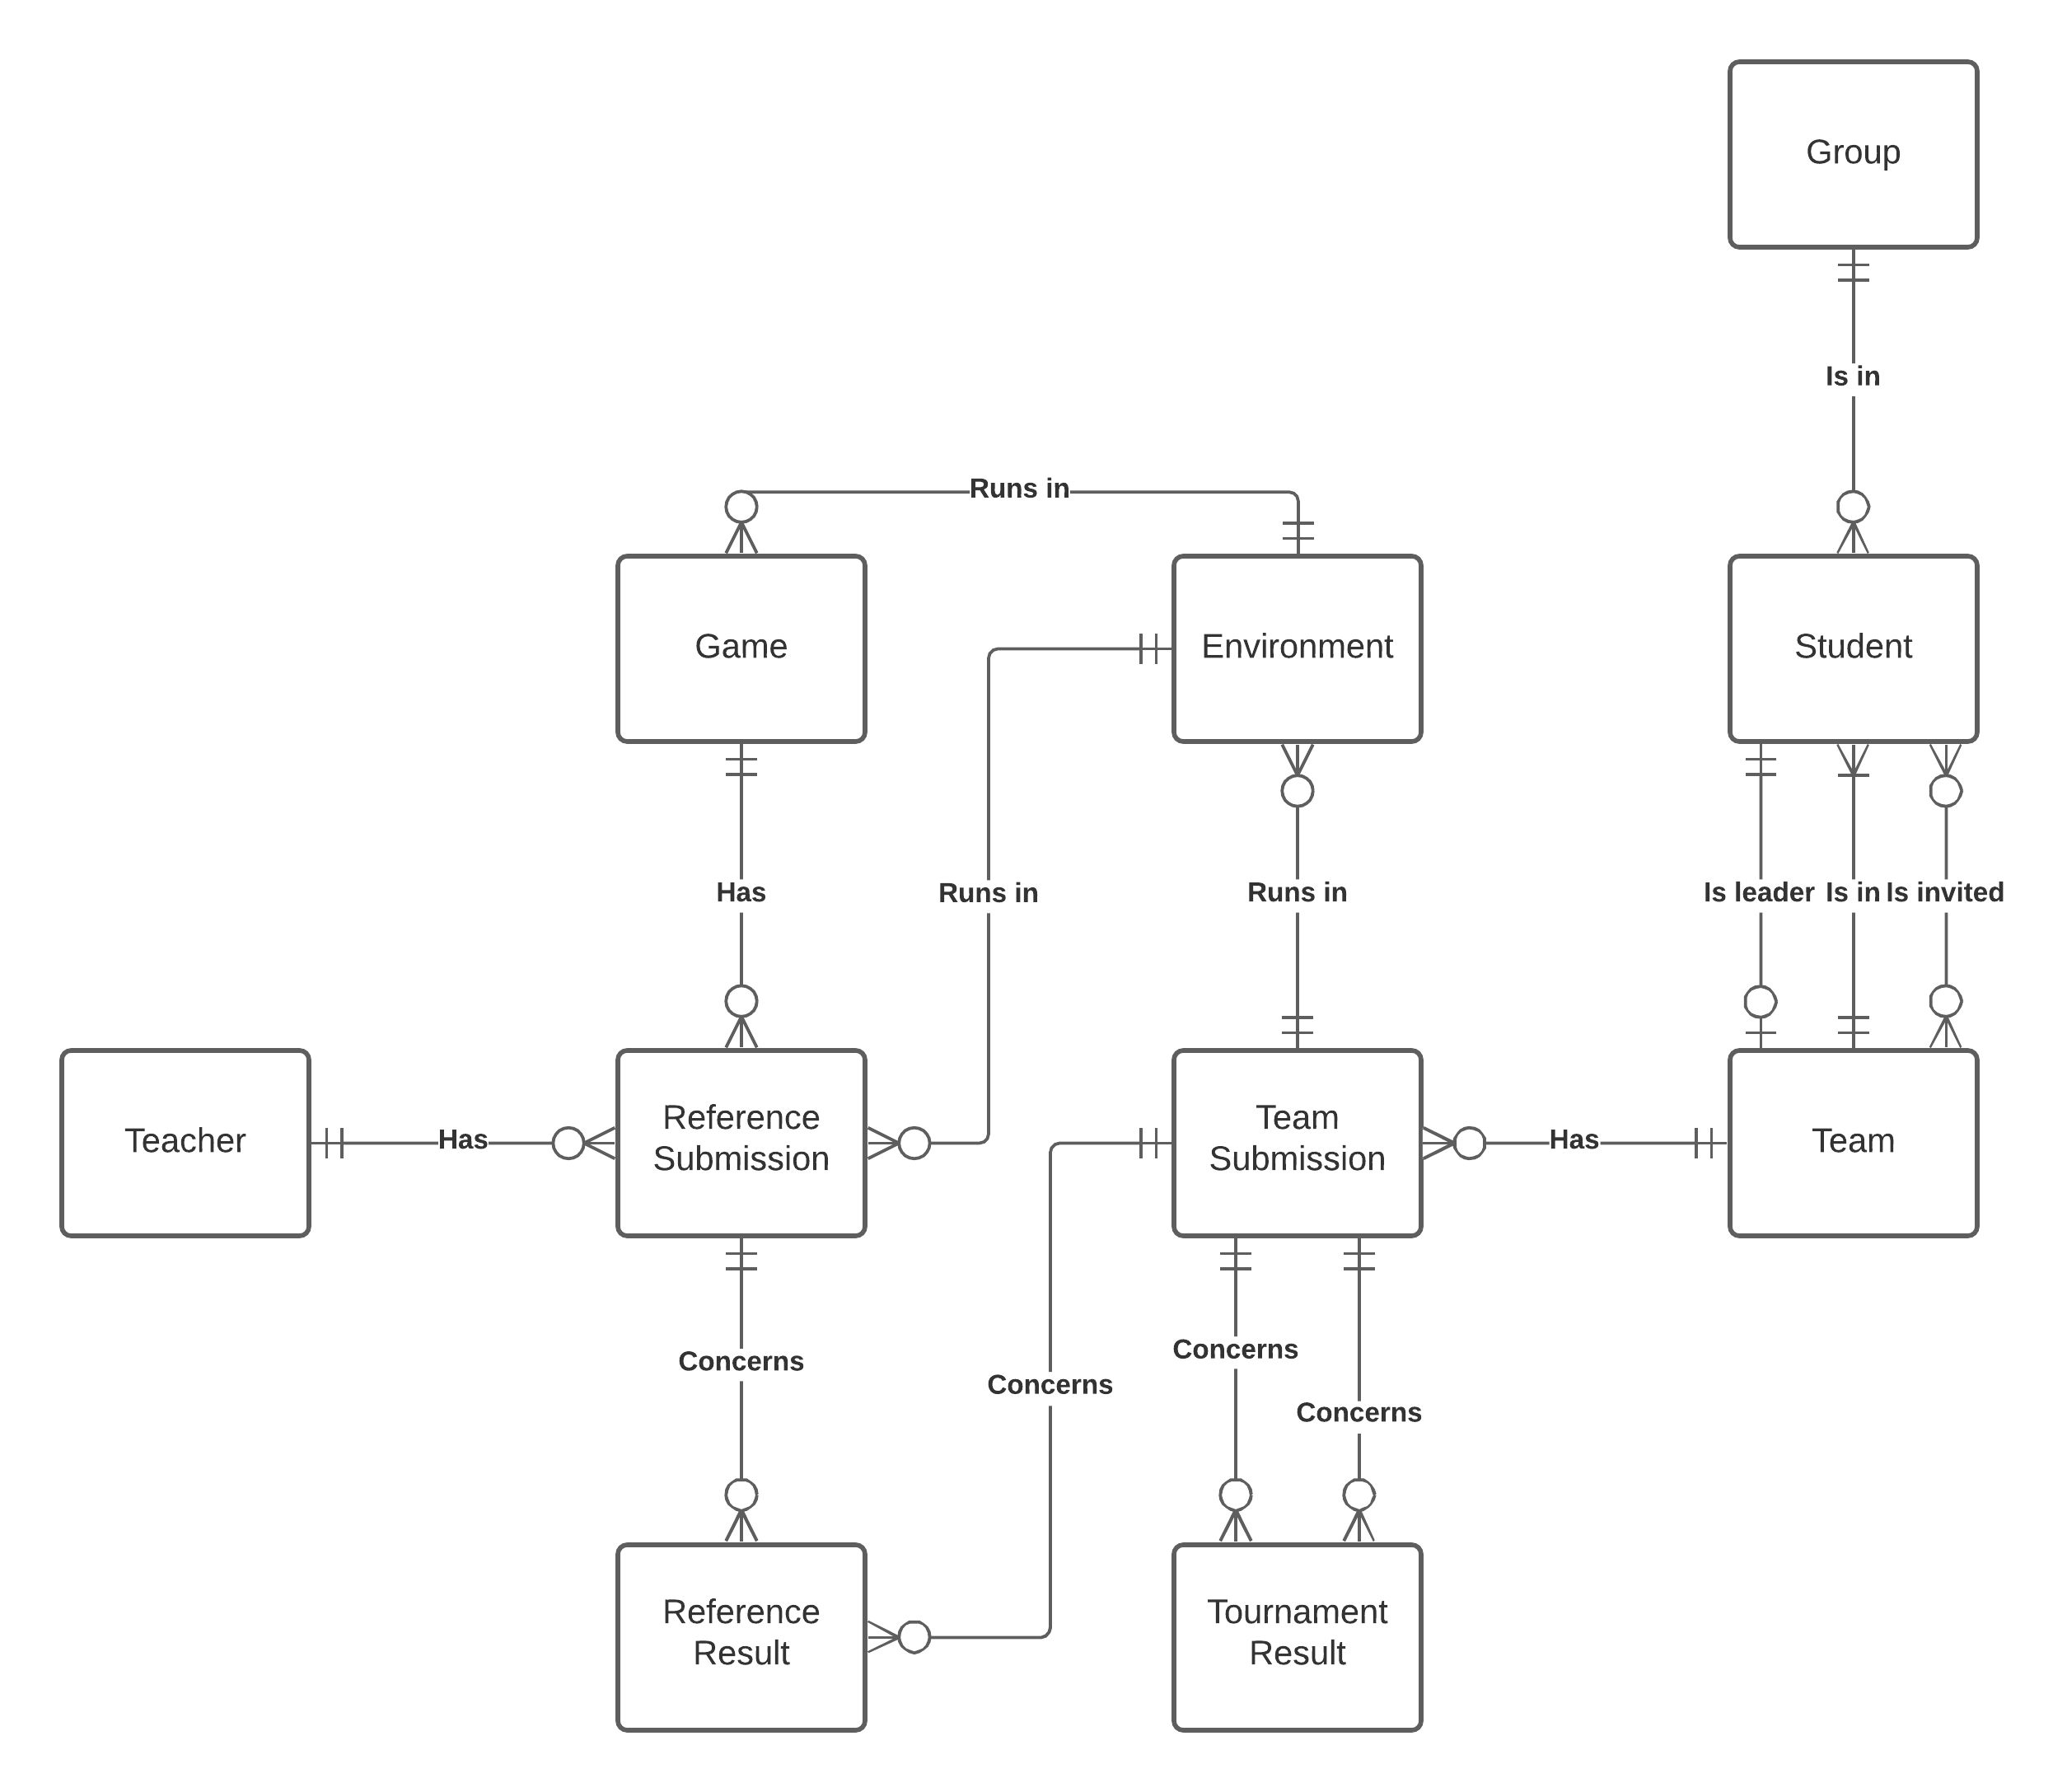
\includegraphics[width=\textwidth]{figures/erd_diagram.png}
    \caption{Entity-relationship Diagram.}\label{fig:er_diagram}
\end{figure}

\subsection{Database schema}
After successfully creating the entity-relationship diagram, we had to transform it into the relational model and then implement it. Most of the relationships between entities in our schema are of 1:n cardinality, which means they did not require a separate relation to be created, other than two relations representing the entities. We mapped the primary key attributes of the relation with ``one'' cardinality as foreign key attributes of the relation with ``many'' cardinality. Other than that, there were some obstacles we came across. 

The biggest issue was how to model three different associations between the student and the team: team invitations, team members and team leader. Since the team invitations relationship is a binary relationship with M to N cardinality, it was apparent that we had to create a separate relation with foreign keys from both student and team relations. Next, since being a team member has 1:n cardinality, we could add a foreign key to a student relation and create a separate relation containing information about team leaders. However, this solution would make our system hard to extend if we wanted to allow the user to participate in multiple teams. In the end, we chose to create a separate relation for information about team members with a foreign user id key in the teams table. We decided that the solution that makes adding new functionalities easy is the best one. 

Another dilemma we came across was whether to use natural or surrogate primary keys since the decision usually varies depending on the case. After going through the advantages and disadvantages of both of these solutions applied to our system, we came to the conclusion that using surrogate keys for our tables would be the best choice.

In the beginning, natural keys seemed like the most logical choice, since most of the tables in our database already had variables that had to be unique. It turned out that this solution could introduce many problems in the future. Natural keys are volatile, which means that even though some variables used as a primary key are unique, they might still require changing in the future. For instance, if we set the team name as a primary key for the ``teams'' table, modifying it would require not only an update in the ``teams'' table but also updates in all the tables that are associated with that table and are using team name as a foreign key. Surrogate keys never need to be changed because there is no meaning associated with them outside of our system, so the problem mentioned is non-existent.

On the other hand, retrieving information from multiple tables connected using surrogate primary keys might require executing more JOIN operations. This problem should not affect our system, though, since we usually need more than just a child table's unique name when retrieving information, so these operations are inevitable. Additionally, surrogate keys, being almost always integers, typically require only 4 bytes to store, meaning the primary key index will be smaller in size, allowing better performance for the mentioned JOIN operations. 

After considering all of the potential solutions, the relational diagram was created, as seen in figure~\ref{fig:relational_diagram}

\begin{figure}[t]
    \centering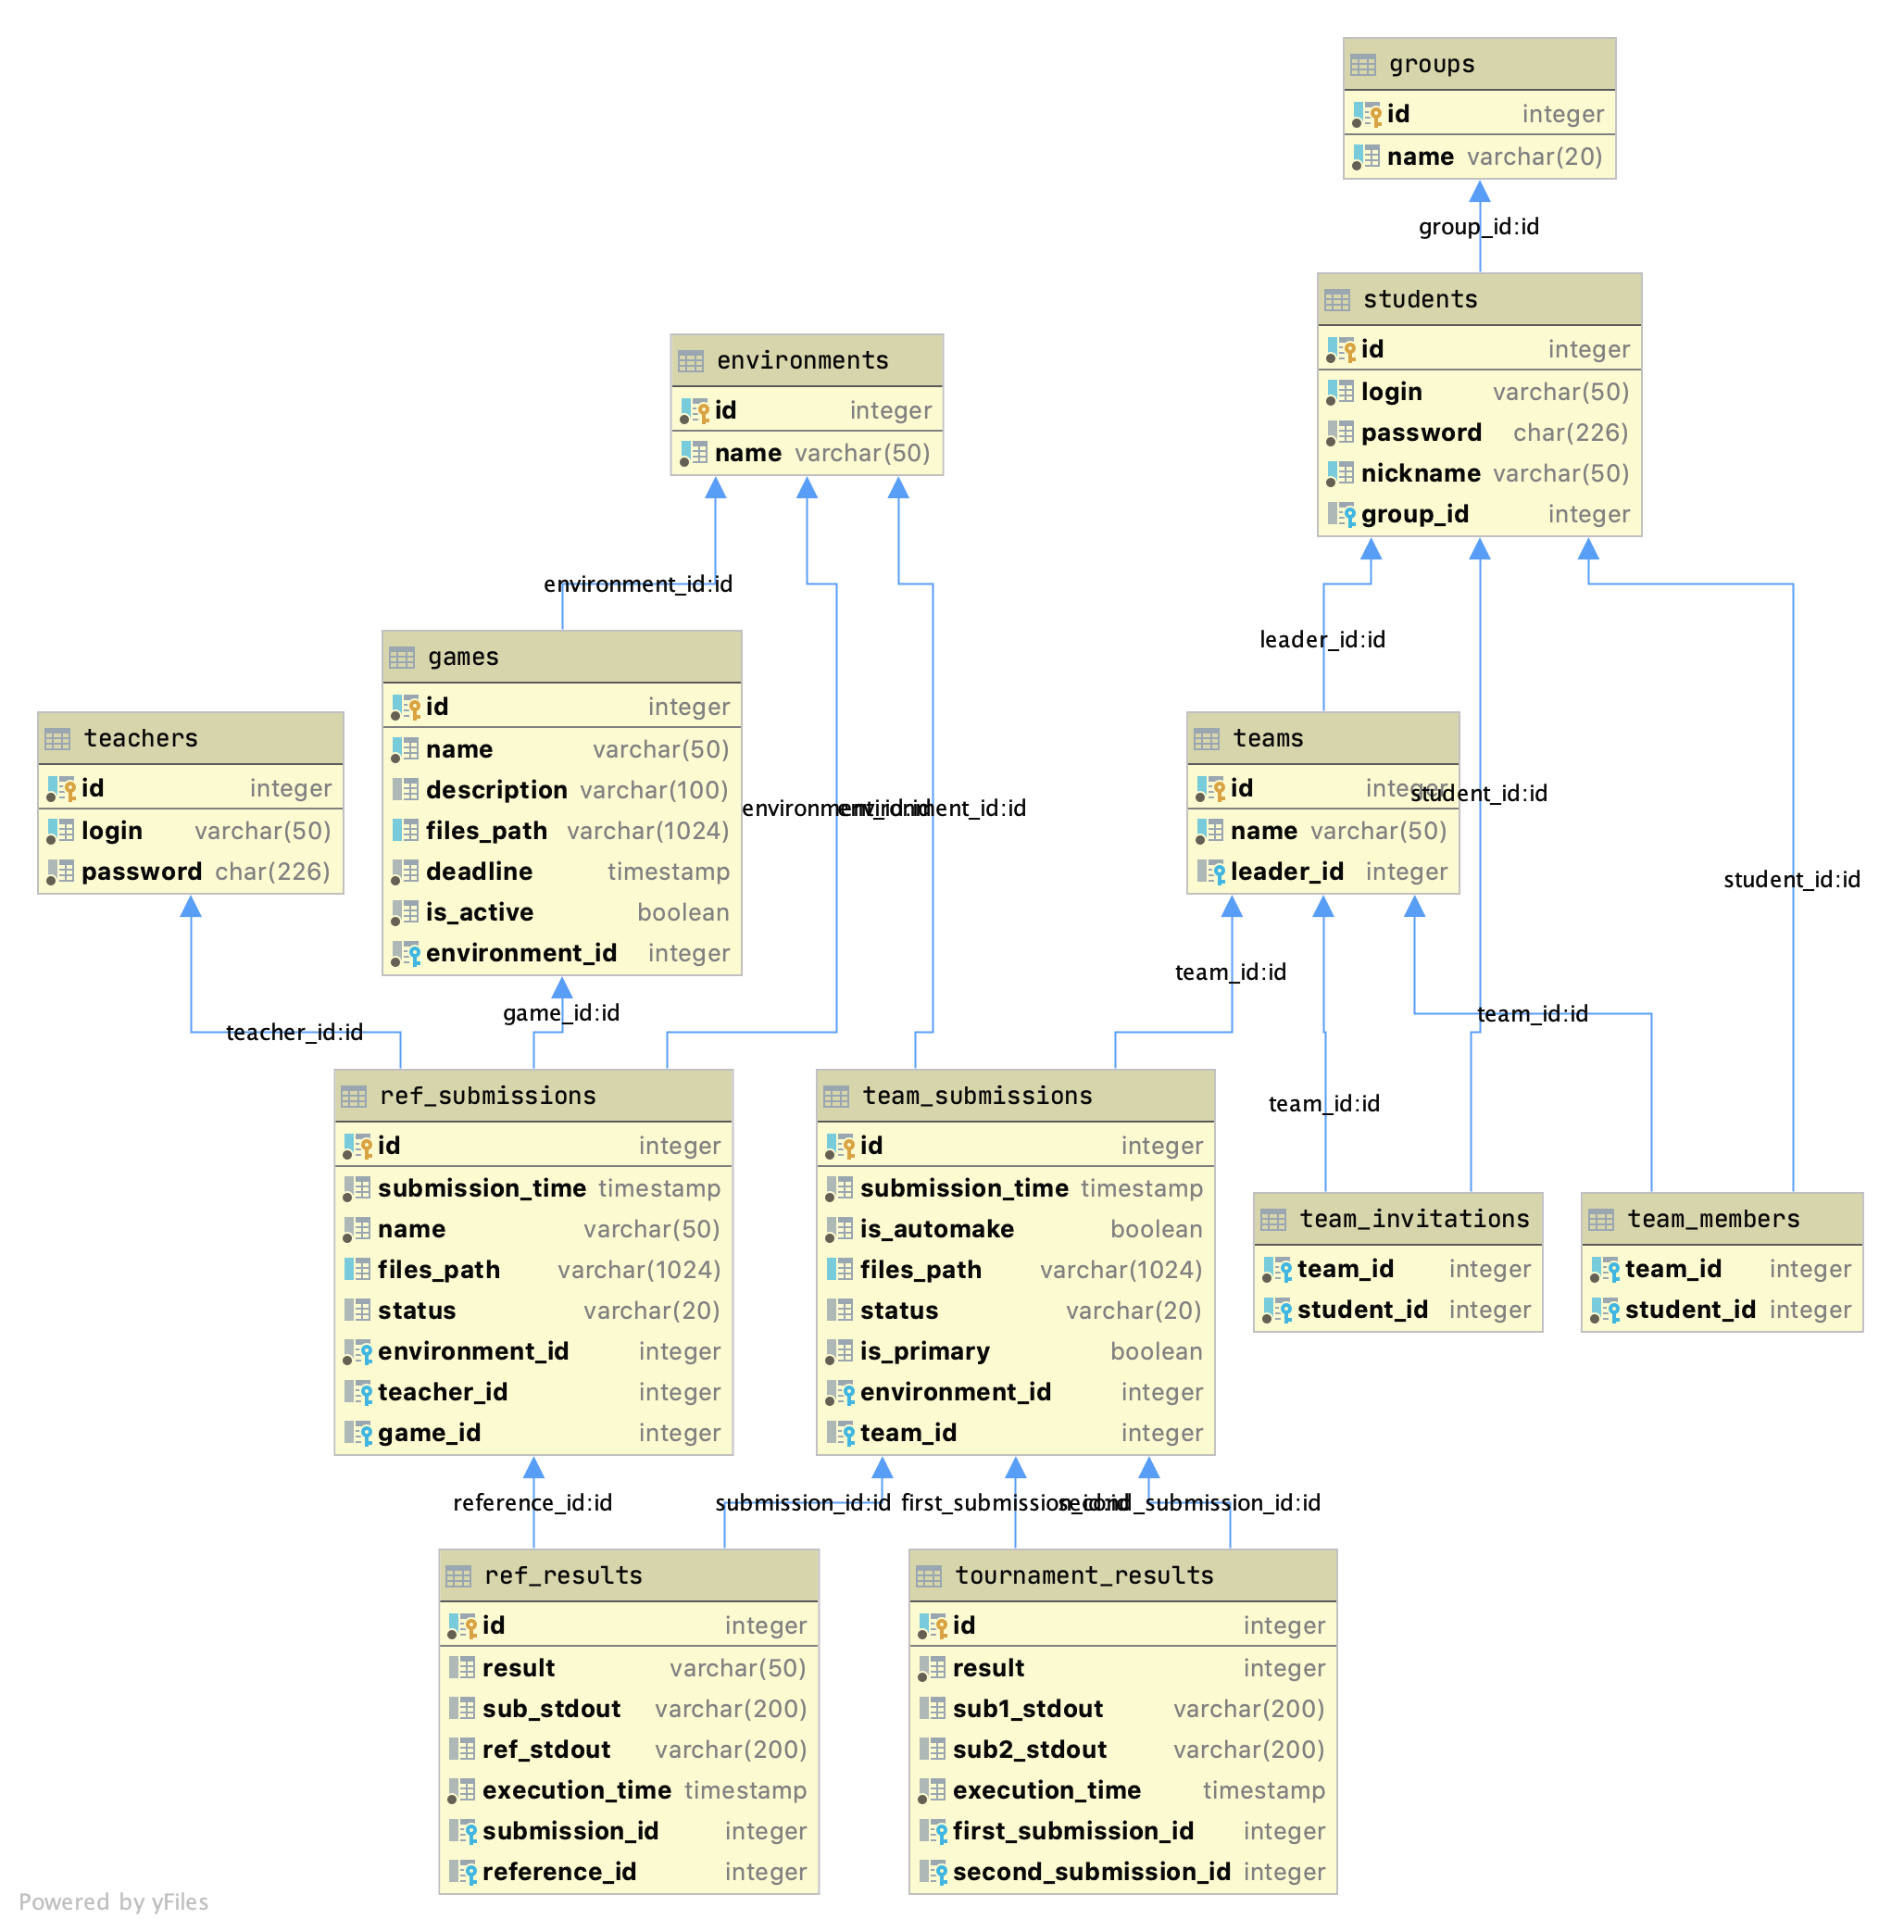
\includegraphics[width=\textwidth]{figures/relational_schema.png}
    \caption{Relational Diagram.}\label{fig:relational_diagram}
\end{figure}

\subsection{Database stored procedures and triggers}

In the process of creating the database, we realised that correctly defining the database schema itself would not be enough to ensure that specific requirements are fulfilled. Those requirements came down to maintaining the integrity of student teams and their submissions. We had to make sure that:

\begin{itemize}  
\item a student is in a team at all times (even if the team consists of only one person),
\item a team always has a leader,
\item the newest submission is the one chosen for the evaluation unless the leader decides otherwise
\end{itemize}

To guarantee that those conditions are met, we made use of procedures and triggers provided by PostgreSQL. Another approach we could take was to implement those in the backend API code. However, this approach would be prone to redundant code replication with multiple functions needed to perform the same database operation. We wanted to make sure that a single user team will be automatically created both when a new student joins the competition and when any student leaves his current team, without worrying about it too much in the API. The stored procedures are also much quicker than executing a series of SQL queries in the backend code.

\section{API}
\subsection{Technologies}

% Framework choice (FastAPI vs Flask vs Django) 
% FastAPI automatic REST documentation & testing site

The first and most important decision we had to make was choosing the web framework we would work in. There are many available frameworks for Python application development, and it is vital to keep in mind that the choice of the framework will affect our work's efficiency. Until now, the most popular and widely used Python frameworks were Flask~\cite{flask} and Django~\cite{django}. Even though these are both solid choices, ultimately we settled on a relatively new framework, that surpasses them both in various ways -- FastAPI~\cite{fastapi}. 

Above all, FastAPI is, by the time of writing, one of the fastest Python framework available~\cite{fastapi_benchmarks}; with only Apidaora~\cite{apiadora} above it, while Flask and Django did not even make it to the top ten. In the context of our application, improving the speed of the underlying framework is crucial, knowing that the system might get very busy by the end of the semester. One of the reasons for its speed is that FastAPI has an out of the box, native support for asynchronous code using basic Python keywords: async and await. Using asynchronous requests means that waiting for the result of the game in our system does not stop all the other operations and other endpoints could still be processed, while the system waits for an answer. We did not hesitate to use that to our advantage in the project while implementing communication with the compute server. FastAPI team also claims~\cite{fastapi} that their framework has significantly increased the speed of development, which turned out to be of great importance, considering the development time of our application could not exceed four months. It is also worth noticing that FastAPI team, knowing their framework is relatively new, provided very extensive documentation with many useful examples, which even further sped up our work. FastAPI is also the only framework out of the mentioned that supports up-to-date, automatically generated, interactive OpenAPI (Swagger)~\cite{Haupt2014} documentation. This was crucial in the early stages of development when the backend server was not yet integrated with the frontend application and testing the server alone proved to be inconvenient.

% Environment Anaconda - do instalacji odpowiedniej pythona, paczek i redisa
% Make - simple set up

For proper package and environment managing, we settled on Anaconda. Anaconda uses the concept of creating isolated environments to keep different libraries separate, while also keeping track of their different versions. This way, setting up correct versions of Python and the necessary libraries was made really easy, coming down to installing and activating the environment prepared earlier. Another viable option was Pip, though it turned out that unlike Anaconda it does not offer package binaries installation. This possibility later allowed us to install Redis service on a dedicated Anaconda environment. Using Anaconda had also made our work more manageable in the early stages of development when each person was simultaneously working on different parts of our application. After preparing the necessary environment and dependencies, we use Make utility to provide a simple launch of our application without the knowledge required to set it up.

% Database connection - why noORM (write SQL)
% (Pugsql - Sqlalchemy Core)

For the connection with our database, we decided to abandon the ORM (object-relational mapping) approach in favour of an anti-ORM approach -- PugSQL~\cite{pugsql}. PugSQL is essentially a wrapper built on top of the well-known, lightweight query builder -- SQLAlchemy-core. SQLAlchemy~\cite{sqlalchemy} is a well known Python SQL toolkit that allows efficient data access, and SQLAlchemy-core is its part focused around tables, keys, and index structures without the ORM focused more on the business objects. PugSQL offers a clean separation of SQL and Python code by allowing its users to define database functions using parameterised SQL files. This means that as opposed to the ORM approach, there is no need to create many unnecessary, bulky classes to represent our database in the backend API; instead, we can use the previously written queries. By allowing to store the SQL code in multiple files, PugSQL also gives its users a possibility to manage SQL files in a consistent way. 


% Pydantic Models - automatic request data validation (używamy typing - Optional)

For data validation, we use Pydantic~\cite{pydantic}, a library that is natively available in the FastAPI framework. Pydantic makes validation easy, and when set up correctly, provides automatically sent, easy to understand errors. By choosing the correct data types in pure Python, we provide the information about the types of data we expect to Pydantic, guaranteeing the defined types and constraints in the output model. This makes the data validation very intuitive without the need for learning any new language or library syntax. Pydantic also offers more complex field types with different properties and validation. In our project, we often used the ``Optional'' property, which informs Pydantic, that the chosen model attribute can accept None type apart from the required type. Pydantic also offers custom and more complex validation using the validator Python decorator. We applied this mechanism to create a reusable string validator, which checks if the string is empty or filled with white spaces.

% Uvicorn as server (wiele procesów odpowiadających na zapytania) - w przyszłości NGINX z proxy do Uvicorna (+ load balancer)

Currently, there is one backend application server instance set up, using Uvicorn~\cite{uvicorn}. Uvicorn is a fast Asynchronous Server Gateway Interface (ASGI) server used underneath by FastAPI. ASGI is a standard introduced as an alternative to WSGI (Web Server Gateway Interface), meant to provide an interface between asynchronous Python web applications and frameworks. Uvicorn has many great behaviours implemented to ensure a good connection such as HTTP pipelining, which allows queueing up HTTP requests or default Server and Date headers added to all outgoing requests. 

In the future, Uvicorn should be run behind Nginx, which would act as a reverse proxy for our application. That means that the additional server will be the one communicating with the client and then forwarding the requests to our web server while providing additional features.
Nginx server could improve our servers traffic by compressing the data passed or by caching commonly requested resources. If required, it would also be possible to run multiple backend API instances and use Nginx as an HTTP load balancer to distribute requests and improve our application's performance. Nginx offers many load-balancing methods to choose from together with testing the upstream servers using health checks.

% Redis for session storage (why / simpler viable alternatives)
%session vs token based?

For session storage, our application uses Redis~\cite{redis}. Redis is a database, which features make it perfect for storing sessions. Because it is an in-memory key-value store, as the name suggests, it performs all operations in memory, which makes both reads and writes very fast. Additionally, Redis has a snapshot mechanism implemented by default, which provides a reasonable level of persistence. Another viable solution we considered was using shared memory in Python, but it would shut off the possibility of running multiple backend API instances with common token storage. We would then also have to implement some kind of memory persistence mechanism ourselves in order to prevent the loss of data.

% HTTX do asynchronicznych requestów wychodzących do serwera obliczeniowego

To communicate with the compute server, we use HTTPX~\cite{httpx}. HTTPX is an HTTP client that provides support for both synchronous and asynchronous APIs. Using the asynchronous client, we were able to establish communication with our asynchronous compute server directly. This means when we send the submission for grading, while the compute server has not finished, we can still do some other work. As a result, our application became much more responsive, and its performance was greatly enhanced. It is also worth mentioning that HTTPX offers timeout configuration for each request. We did not hesitate to use those in our compute server requests, which makes our backend API more patient in case of more complex bot algorithms.

% TOML configuration - easy (why not JSON / YAML)
% - JSON - hard to write for humans (not as hard as XML)
% - YAML - complex grammar, insecure, easy mistakes (inconsistent indentation)

Our backend API has a very clear and easy-to-use configuration file, created using TOML~\cite{toml} format. Two other prevalent configuration file formats we considered were JSON and YAML~\cite{yaml}, but both proved to be less effective. JSON is an excellent format for storage and data exchange, as it is relatively easy to read and write, though it lacks some features when it comes to configuration. First of all, JSON is a data-only format, so it does not support comments, which seem vital to understand the configuration. There are some workarounds to include this functionality, but they seem excessive. Furthermore, even though JSON is easy to process for the machines, writing the configuration in this format might make it less transparent and prone to errors, considering the number of braces, commas and quotation marks. Yaml, on the other hand, has better human readability and writability and does not require as many symbols in its syntax. YAML's main disadvantage is its interpretation of the indentation levels, which may prove troublesome and prone to human error. Another downside is its complex grammar, which may prove ineffective in our case. We ended up using TOML because it has a straightforward and easy-to-read syntax, supports comments and does not require indentation like YAML, so there is no room for error.

% Na Voidzie autostart serwera to skrypt, który trzeba podlinkować do /var/services (RUNIT)

\subsection{Endpoints}

% - who has access to which resources (CRUD)

Our application has two main groups of users: teachers and students, each with different types of access to various resources in our database. Defining the terms of these permissions was key to the security of our application. To make sure those terms are clear to us and to achieve a certain level of agreement, we came up with a CRUD (create, read, update and delete) diagram seen in figure~\ref{fig:crud_diagram}. The diagram does not include the results of games as those are created and managed by the API itself with the moment of submission, and the teachers and users can only read them after the system evaluates the solutions. The results are reset automatically after the semester when the teacher activates a new game.

\begin{figure}[t]
    \centering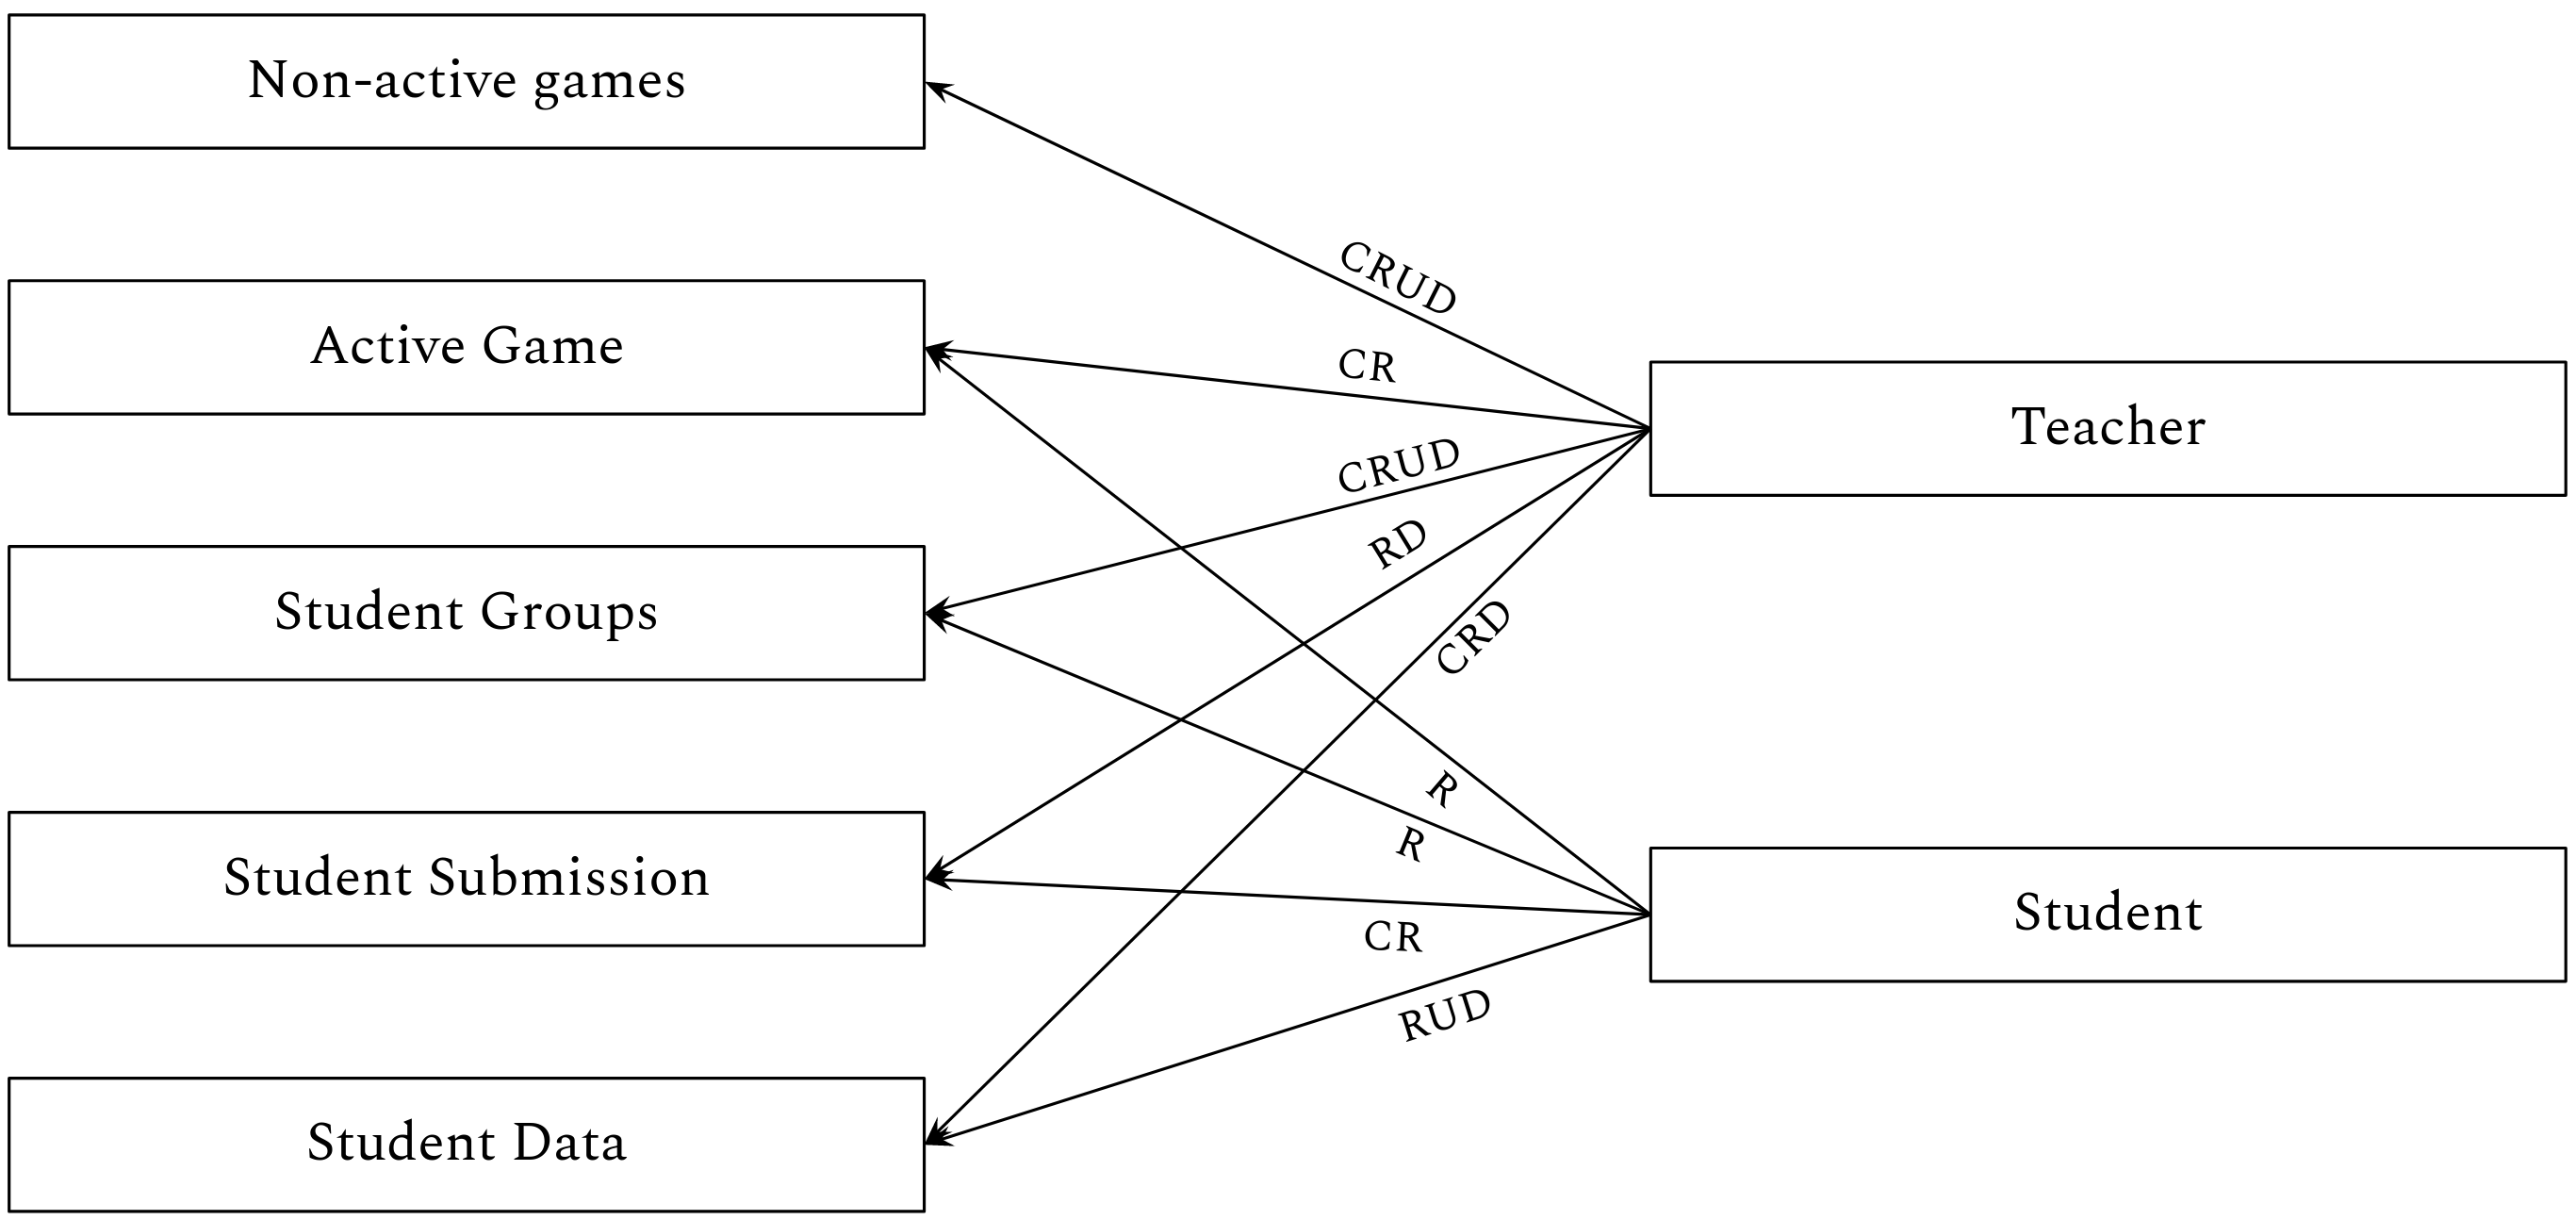
\includegraphics[width=\textwidth]{figures/CRUD.png}
    \caption{CRUD Diagram.}\label{fig:crud_diagram}
\end{figure}

% Endpoint description
% - student endpoints
% - teacher endpoints
% - public endpoints
% Stateful semantics
% - /login to acquire token

The HTTP requests we used in our application are: GET, POST, PATCH and DELETE. Knowing that we will not be updating any resource in its entirety, we decided to refrain from using the PUT request in favour of PATCH.

Before getting access, every user has to authenticate himself using the \tw{\slash login} endpoint. Only then, the system can verify if the user is authorized to use certain functionalities. This feature is further discussed in the security section of this chapter. Using this mechanism, we divided our endpoints into three categories: public endpoints, student endpoints and teacher endpoints as seen in tables~\ref{tab:public_endpoints},~\ref{tab:student_endpoints}~and~\ref{tab:teacher_endpoints}, respectively. Note that the lower part of table~\ref{tab:student_endpoints} is accessible only to the students with an additional team leader role. The API checks if the user identified by the session token is the leader of his team. If not, the ``FORBIDDEN'' HTTP exception with 403 status code is returned.

\begin{table}[t]
\caption{Overview of the public API endpoints with a short description.}
\label{tab:public_endpoints}
\centering\footnotesize
\begin{tabular}{p{0.1\linewidth} p{0.30\linewidth} p{0.50\linewidth}}
\toprule
Method & Endpoint & Description \\
\midrule
POST & \tw{/login} & Authenticate the user, identify its role and return the token \\
GET & \tw{/groups} & Obtain ids and names of groups \\
GET & \tw{/environments} & Obtain ids and names of environments \\
GET & \tw{/games/active} & Obtain the information about the currently active game \\
GET & \tw{/games/active/widget} & Retrieve an interactive widget of the currently active game \\
\bottomrule
\end{tabular}
\end{table}

\begin{table}[t]
\caption{Overview of the student API endpoints with a short description.}
\label{tab:student_endpoints}
\centering\footnotesize
\begin{tabular}{p{0.1\linewidth} p{0.30\linewidth} p{0.50\linewidth}}
\toprule
Method & Endpoint & Description \\
\midrule
GET & \tw{/students/me} & Obtain the information about the logged-in student \\
PATCH & \tw{/students/me} & Update the information about the logged-in student \\
DELETE & \tw{/students/me} & Remove the logged-in student's profile \\
GET & \tw{/students/me/invitations} & Obtain team invitations of the logged-in student \\
POST & \tw{/students/me/invitations/ \{team\_id\}/accept} & Change the team of the logged-in student and remove the invitation as long as the invitation to that team exists \\
POST & \tw{/students/me/invitations/ \{team\_id\}/decline} & Remove the logged-in student's invitation to the chosen team as long as this invitation exists \\
GET & \tw{/students/me/team}
 & Obtain the information about the logged in student's team \\
POST & \tw{/students/me/team/leave} & Remove the logged-in student from the current team and automatically create a new one-member team with the student as the leader \\
GET & \tw{/team/\{id\}/members} & Obtain the members of the logged-in student's team \\
GET & \tw{/team/\{id\}/invitations} & Obtain the sent invitations of the logged-in student's team \\
GET & \tw{/teams/me/submissions} & Obtain the information about the logged-in student's team submissions \\
POST & \tw{/teams/me/submissions} & Submit a new submission on behalf of the logged-in student's team \\
\bottomrule
PATCH & \tw{/team/\{id\}} & Update the information about the logged-in student's team \\
PATCH & \tw{/teams/\{team\_id\}/leader/ \{leader\_id\}} & Update the leader of the logged-in student's team \\
POST & \tw{/teams/\{team\_id\}/invitations/ \{nickname\}} & Invite a new student to the logged-in student's team \\
DELETE & \tw{/students/\{team\_id\}/invitations/ \{student\_id\}} & Remove an invitation to the logged-in student's team \\
POST & \tw{/teams/me/submissions/primary/ \{id\}} & Set the chosen submission as the primary submission of the logged-in student's team \\

\bottomrule
\end{tabular}
\end{table}

\begin{table}[t]
\caption{Overview of the teacher API endpoints with a short description.}
\label{tab:teacher_endpoints}
\centering\footnotesize
\begin{tabular}{p{0.1\linewidth} p{0.30\linewidth} p{0.50\linewidth}}
\toprule
Method & Endpoint & Description \\
\midrule
POST & \tw{/students} & Create a new student profile \\
POST & \tw{/teachers} & Create a new teacher profile \\
POST & \tw{/groups} & Create a new student group \\
PATCH & \tw{/groups/\{id\}} & Update the information about the chosen student group \\
DELETE & \tw{/groups/\{id\}} & Remove the chosen student group \\
GET & \tw{/games} & Obtain list of the games \\
GET & \tw{/games/\{id\}} & Obtain the information about the chosen game \\
POST & \tw{/games} & Create a new game \\
PATCH & \tw{/games/\{id\}} & Update the infomation about the chosen game \\
DELETE & \tw{/games/\{id\}} & Remove the chosen game \\
POST & \tw{/games/activate/\{id\}} & Make the chosen game active \\
POST & \tw{/games/\{id\}/ref\_submissions} & Create a new reference bot for the chosen game \\
\bottomrule
\end{tabular}
\end{table}

% data validation mention

As we mentioned earlier for data validation, we used Pydantic. In case of an incorrect data entry, the system detects an error during the validation and returns an error code with a human-readable message explaining the problem. The web application then captures this message and informs the user about the situation. If a user tries to bypass the Pydantic validation, the database itself will prevent from inserting the data thanks to various constraints set on the tables.

% input file formats - markdown (tabelki, bloki kodu, obrazki) -> kompilacja do HTML
% archives - .zip, .tar, .gzip, ...
% interactive game - .html (can contain JavaScript)

The files accepted by the application can be specified in the TOML configuration. At the time of writing the application accepts not only files specific to the supported programming languages but also zip archives for game and bot executables. In the future, this functionality can be further improved by including other archive extensions. It is also worth mentioning that the teacher can create the overview and rules of the game in the Markdown format, which is compiled to HTML, using Python-Markdown library~\cite{python_markdown_lib} after the upload. This opens up many possibilities for the teacher to conveniently write complex text with easy-to-read tables or blocks of code and even insert images from the internet by simply inserting the URL of an image. The interactive game is passed in an HTML file containing JavaScript code which is then rendered in the web application.
\subsection{Security}

% Session management (teacher vs student token) (session timeout)
To authenticate users, we decided to implement a session-based approach, instead of the token-based, mainly because JWT (JSON Web Tokens) adds unnecessary complexity. As we mentioned earlier, we used Redis for session storage. Before getting access to the application functionalities, the user must authenticate oneself using the /login endpoint. Only if our application recognises the user as one of the students or teachers and confirms that the password is correct, the user may access the corresponding part of the website. At the same time, the user session is created. First, a pseudorandom hexadecimal string is generated and hashed using a SHA256 hash function from the well-known Python hashing library -- Passlib~\cite{passlib}. The output, detailed in the Passlib documentation~\cite{passlib_sha256} then becomes the user's session token. With the new token and expiration time set, a new session entry is created. In the case of a student type user, the session entry additionally keeps track of the latest submission time to limit the number of student submissions per minute. Each time the user tries to access the application, they provide the session token in the HTTP X-SESSION-TOKEN header to authorize access and check the session's timeout. Both token expiration time and submission time limit can be set in the TOML configuration for our application.

% Basic login system (salted hashes, argon2 why?) 
% - gotowe crypto passlib - battle tested

To keep our application safe, we had to implement and secure a basic user login system. In our mechanism, we are using a login and password pair. The algorithm first checks the login and searches in the database for the existing user with that login. Then the system verifies the password against the corresponding hash in the database. Keeping the passwords as plaintext in the database would be a flagrant violation of security. To keep our users' passwords safe from any breaches, we had to pick a hashing algorithm carefully. At the time of writing, the most commonly used encryption algorithms are PBKDF2, Bcrypt, Scrypt and Argon2. We decided not to take PBKDF2 and Bcrypt into account since they can be cracked taking advantage of their low resistance to GPU attacks. Both Scrypt and Argon2 both have additional memory requirements (they are memory-hard), making them more resistant to this kind of attacks. In the end, we decided to choose Argon2, as Scrypt is a much more complex algorithm, the design of which has yet to be fully motivated. Argon2, at the same time, offers three different implementations with various parameters, which gives us more flexibility than Scrypt. The Python library we used is the same we used with session tokens - Passlib~\cite{passlib}. It is worth mentioning that as Passlib documentation states: ``In the near future, it [Argon2] stands likely to become the recommended standard.''~\cite{passlib_argon2}

% HTTPS (let's encrypt) + CORS configuration (dla przyszłej domeny)

Our application is currently hosted only locally, but in the future, we might want to set up our domain with a specific name and our backend API is prepared for this course of action. FastAPI has natively implemented Cross-Origin Resource Sharing (CORS) mechanism. CORS  is a mechanism that can allow our server to choose any domain and port from which it should allow access to the resources. In our application, CORS is already set up, and currently, it only allows the access to the locally run HTTP web application on port 1234. If we were to move our application to a dedicated domain, adding it to the CORS origin list would suffice, where the origin consists of a protocol, domain and port. Once acquiring our domain, it would be worth considering moving from HTTP to HTTPS, since it helps maintain a secure connection between our server and the client's browser. Using Let's Encrypt, the transition will be seamless and much more comfortable than buying the certificate from third-parties. 

\chapter{Compute server}
\label{chap:compute}

\section{Security} %Piotr

In order to enable reliable compilation and execution of user-provided programs on the compute server, it was necessary to separate them from the rest of the
system. If we were to naively compile and execute them without such separation,
the system would be susceptible to various exploits - user programs could try
to influence the execution of the opponent or judge programs, or cause other
system malfunctions and impair the operation of the server, e.g. by accessing
the file system or executing arbitrary programs, potentially as a privileged
user~\cite{Forivsek2006}.  Another concern which necessitated containerization
was the usage of system resources by user programs -- one process could
potentially influence the performance of the rest by allocating all of the
available memory, or using all of the CPU time. To prevent these issues, we
considered various containerization solutions.

% TODO(piotr): discuss containers vs VM?

As the compute server was designed to run under the
Linux~operating~system~\cite{linux}, one possibility was to use the available
kernel features and develop the containerization solution ourselves. The file
system separation could be achieved using \tw{chroot}, access to any
networks, devices and other processes could be restricted using
kernel~namespaces~\cite{namespaces}, and the usage of system resources could be
controlled using cgroups~\cite{cgroups}. This solution would be simpler (in
terms of the resulting system complexity) than the alternatives, which are
implemented using the same kernel features, and probably would allow us to
achieve minimal container overhead.  Minimizing the external dependencies of
the project could also improve portability and maintainability, simplifying the
installation process. On the other hand, it would require more work to develop
an original containerization solution, than to use an existing one, and
developer time was a major limiting factor for this project. Our team did not
have extensive experience in this area prior to this project, and as systems
security is a very vast and complex subject, we would risk having serious
security flaws in our design, which even if detected, would require even more
developer time to fix. For these reasons, we decided to use an existing
solution.

The most widely used container solution at the time of writing this thesis was
Docker~\cite{docker, Flexera19}. The main advantage of using it we considered
was its popularity -- choosing a tool that most engineers are familiar with
would mean, that anyone continuing our work would find it easier to understand
the system. It would also guarantee that the tool is well documented and
tested. However, Docker, in particular, is a very complex toolset, and it
provides a multitude of functionalities that were not necessary, nor desirable
in our project, e.g. it has been designed with the intention of creating
portable container images, which in our case did not provide any advantage and
would have slowed down the creation of the container.  In Docker to create a
container for running a program, all of the program's dependencies have to be
stored within the container image, which would cause unnecessary duplication of
the shared libraries. Docker provides a harder abstraction barrier between the
OS and the container than some of the other alternatives, therefore it would be
harder to adapt it for our use case.

The solution we finally settled on was LXC~\cite{lxc}. It was also a widely
adopted solution, with the advantage of being well documented and tested, but
in comparison with Docker it provided less overhead and was more easily
adjustable. We utilized a custom container template, which allowed the
libraries and programs required for the compilation of the user-provided
programs to be shared between all containers in a read-only manner. One
significant advantage over Docker was that in LXC the container file system is
easily accessible from the parent process, which allowed for a lot of
flexibility regarding the choice of communication medium.

\section{Containers}

To create a container, LXC executes our template script \tw{lxc-player}, which
creates a config file and a rootfs directory that LXC will set as the system
root of the contained processes with \tw{chroot}. This template needs to be
installed on the target system, and LXC needs to be configured appropriately for
the compute server to function correctly. Since the configuration process is
very error-prone we prepared a script which handles it automatically, together
with an instruction for manual installation describing each step.

In the config file created by the \tw{lxc-player} template we use
\tw{lxc.cap.drop} to drop potentially harmful kernel capabilities
\cite{capabilities} like \tw{CAP\_SYS\_MODULE}, which would allow user programs
to load or unload kernel modules, or \tw{CAP\_SYS\_TIME}, which could allow
them to affect system time. Note that this is not the only measure preventing
such security breaches - we designed the template specifically to be run by an
unprivileged user, so even if the list of dropped capabilities was incomplete
accessing such sensitive functionality should remain impossible.

The \tw{lxc.mount.entry} directive is used to set directories which are shared
with the host.  These are \tw{/bin}, \tw{/sbin}, \tw{/lib} and \tw{/usr}. They
are mounted by LXC when the container is started so that all of the necessary
build tools, environments and their dependencies are accessible from the
containers. We decided to add one additional directory for utility scripts and
TinyBuffers library files as \tw{/share}. All of the directories are mounted
read-only.

The resource limits are configured using \tw{lxc.cgroup}. The cgroup file system
is mounted by LXC automatically and all the necessary controllers configured.
In our configuration, the memory usage is limited to 512 MiB per container and
an equal split of the CPU resources between all the containers is ensured.

% TODO(piotr): the cgroup section is undercooked

To prepare the rootfs directory and make sure all programs function properly
within the container all the necessary system directories are created (that is
\tw{/bin}, \tw{/dev}, \tw{/etc}, \tw{/home}, \tw{/lib}, \tw{/proc}, \tw{/root},
\tw{/sbin}, \tw{/sys}, \tw{/tmp}, \tw{/usr}, \tw{/var} and \tw{/share}). A
temporary file system is mounted to \tw{/tmp} automatically by LXC when the
container is started. To finish the system configuration an empty
\tw{/etc/fstab} file is created, as well as \tw{/etc/passwd} and
\tw{/etc/group} files, filled in with the simplest possible data for a root
user group and account.

Finally, the player files and communication channels are prepared. All files
from the directory to which player files were uploaded are copied into
\tw{/root} and two named pipes, \tw{/root/fifo\_in} and \tw{/root/fifo\_out}
are created.

After the template file is installed on a system, containers using it can be
created with \tw{lxc-create -n CONTAINER\_NAME -t player}. Parameters to the
template are given after \tw{--} at the end of the command line. The directory
with player files can be specified with \tw{--copydir=DIRECTORY}, with
\tw{DIRECTORY} substituted appropriately. Similarly, the rootfs location and the
directory to be mounted as \tw{/share} can be specified with
\tw{--rootfs=DIRECTORY} and \tw{--sharedir=DIRECTORY} respectively.

To test whether the configuration was correct a \tw{bash} shell can be opened
within a given container by executing \tw{lxc-execute -n CONTAINER\_NAME -- bash}.

\section{Supervisor}

The compute server API is exposed via the HTTP protocol by a Python program
which we called the supervisor. Most of the web technology stack
is the same as in the case of the database server. We used the same web
framework, that is FastApi, the requests are handled asynchronously, and the
configuration of the server is stored in TOML format. In this case, it was not necessary to
use a Redis database for session data, so we decided to use a simpler
scheme utilizing shared memory instead. We used Gunicorn~\cite{gunicorn} to set
up shared resources before the fork. To prevent unauthorized access to the
compute server API we set up Cross-Origin Resource Sharing (CORS), with allowed
origins easily configurable in the TOML config file. Also, as a second safety
measure, we require an API token to be sent with the request; the token is also
configurable in the TOML file and can be set individually for each instance of
the supervisor. In the current configuration, there is only one instance,
running on the same host as the database server, however, when eventually they
will be moved to separate hosts, it may be worthwhile to consider moving from
HTTP to HTTPS and using Let's Encrypt for certification as mentioned in
chapter~\ref{chap:database}. Such measures would not be necessary if the
compute servers wouldn't have access to the global network.

All the endpoints of the supervisor API are listed in
table~\ref{tab:supervisor_api}.

\begin{table}[t]
\centering\footnotesize
\caption{Supervisor API endpoints.}
\label{tab:supervisor_api}
\begin{tabular}{l l l}
\toprule
Method & Endpoint & Description \\
\midrule
GET & \tw{/job/\{id\}}         & Query the execution status of a job \\
PUT & \tw{/job/\{id\}}         & Create a job with the given id \\
PUT & \tw{/player/\{id\}}      & Submit a new player \\
PUT & \tw{/ref\_player/\{id\}} & Submit a new reference player \\
PUT & \tw{/game/\{id\}}        & Submit a new game judge program \\
\bottomrule
\end{tabular}
\end{table}

The endpoints for submitting a game judge program, player or a reference player
are very similar. Parameters that need to be provided are \tw{env\_id} -- the
execution environment id of the given program as described in the
chapter~\ref{chap:database}, and \tw{data} -- an archive with the program files
or a single text file with the source code. The \tw{/player/\{id\}} and
\tw{/ref\_player/\{id\}} also take an optional parameter \tw{automake} which if
set to \tw{true} enables a system which tries to automatically detect how the
program files should be built -- a convenience feature mainly meant for simple,
one file programs. The \tw{/ref\_player/\{id\}} endpoint also requires a
\tw{game\_id} parameter.

When uploading the archive with a program source to either endpoint without
using the \tw{automake} feature, the archive is expected to contain an
executable (most likely a bash script) called \tw{build}, which will compile
the source code if any compilation is necessary. In the case of programs in
interpreted languages like Python such file is not necessary. When executing
the compiled program it is expected that the resulting directory contains an
executable called \tw{run}, so either the \tw{build} script has to output the
executable with this name, or the archive has to contain a separate \tw{run}
script for running the program.

To initiate a game between two chosen players, a job has to be created. The
parameters required by this endpoint are the \tw{game\_id}, identifiers of the
players \tw{p1\_id} and \tw{p2\_id}, and an optional parameter \tw{is\_ref}
which should be set to \tw{true} when \tw{p2\_id} designates a reference
player. The server will respond to this request with game results after the
game has finished; in the meantime, the status of the job can be queried with
GET \tw{/job/\{id\}}.

The judge program is expected to print the result of the game in the final line
of output. All the possible outputs are listed in table \ref{tab:judge_result}.

\begin{table}[t]
\centering\footnotesize
\caption{Allowed judge program outputs.}
\label{tab:judge_result}
\begin{tabular}{l l}
\toprule
Output & Description \\
\midrule
\tw{WINNER X}  & Player X has won (X can be either 1 or 2) \\
\tw{TIMEOUT X} & Player X failed to commit a move before timeout (X can be either 1 or 2) \\
\tw{CHEATER X} & Player X did not conform to the game rules (X can be either 1 or 2) \\
\tw{DRAW}      & The game was a draw \\
\bottomrule
\end{tabular}
\end{table}

\section{Testing}

The compute server, as described above, consists of many interconnected
components, which interact in complex ways and configuration of any of the
components could potentially cause a failure of the whole system -- even if in
separation from the system it would seem correct. For this reason, we identified
testing of the system as a whole to be essential.

To achieve a reproducible testing environment, we prepared a virtual machine
with Void~Linux~\cite{voidlinux} installed and all the necessary packages
configured. We had chosen this Linux distribution specifically because it has a
very minimal set of packages installed by default, which helped us to avoid
hidden dependencies, made the configuration more easily transferable to other
Linux distributions and lowered the virtual machine size. Also, members of our
team had extensive experience working with this distribution earlier, so it was
naturally the preferred choice.

The most sensitive element of the configuration which failed repeatedly and
proved hard to debug was LXC. It required altering of multiple global
configuration files, dealing with erroneous behaviour of some versions of its
dependencies, inconsistent behaviour across different Linux distributions,
problems specific to distributions using systemd \cite{systemd}, and loading
necessary kernel modules on some systems. All of these problems inspired us to
create a script for automatic configuration of LXC specifically for the use of
our container template.

Other necessary project dependencies which were installed on the virtual
machine included PostgreSQL, Python3 and Node.js, which were used to test the
supervisor in conjunction with the database server and the web application.

To automate the testing of supervisor endpoints we prepared a set of
scripts using \tw{curl}~\cite{curl} which tested many potential failure
scenarios by verifying the response of the server for certain requests. We also
tested the functioning of the compute server in conjunction with the database
server and the web application, by manually going through the use cases. We did
not find the available GUI automated testing options to be robust enough to
warrant employing such solutions.


\chapter{Case study -- Pentago}
\label{chap:pentago}

\section{Game overview}

In the process of developing the AI Colosseum, we considered it crucial to also
develop an example game and bots, to test the whole system in practice. Having
such an example helped to expose the limitations of the design and improve it.
It also helped to document the intended use of the system, providing a
reference for any future developers. The game we have chosen to implement was
Pentago~\cite{pentago}. We selected it mainly because this game was already used in the AI
course, so it would probably be the most useful and would enable us to make
quantifiable comparisons between the old and the new system, but also because
it's rules are relatively simple, and we thought it would make for a good
example.

Pentago is a modern, two-player board game. It is a variation of a 5-in-a-row
game, played on a $6 \times 6$ board, where each player must rotate one of the
board quadrants by 90 degrees in any direction, after placing a stone. The
rotation is compulsory unless the player achieves the winning condition
immediately after placing the stone. Since the rotation allows multiple
5-in-a-row's to emerge simultaneously, a board position where the winning
conditions of both players are satisfied is considered to be a draw.

Since the rules are based on an m,n,k-game, it's easy to make them more generic
and allow different board sizes. In fact, the previous system defined the rules
in such a way, so we decided to also support them. In the generic version, the
game is played on a $n \times n$ board, where $n \bmod 4 = 2$ and the winning
row length is $k = \frac{n}{2} + 2$.

\section{Judge program}

In AI Colosseum every judge program defines its own protocol to be used with
TinyBuffers over a named pipe as a medium, that player programs have to respect.
In our Pentago judge protocol, it is always the player that initiates a message
exchange. The response for a specific message type is sent with the same tag
back to the player, if it is required. If a message breaking the judge protocol
is ever received from a player, they are immediately disqualified. All the
message types are shown in table~\ref{tab:pentago_protocol}.

\begin{table}[t]
\centering\footnotesize
\caption{Messages used in the Pentago judge protocol.}
\label{tab:pentago_protocol}
\begin{tabular}{l c c c}
\toprule
Name & Tag & Request & Response \\
\midrule
\tw{MSG\_MAKE\_MOVE  } & 1 & \tw{(U8,U8,U8)} & None \\
\tw{MSG\_COMMIT\_MOVE} & 2 & \tw{(U8,U8,U8)} & None \\
\tw{MSG\_GET\_MOVES  } & 3 & \tw{()}         & \tw{(U8[N],U8[N],U8[N])} \\
\tw{MSG\_UNDO\_MOVE  } & 4 & \tw{()}         & None \\
\tw{MSG\_GET\_WINNER } & 5 & \tw{()}         & \tw{U8} \\
\tw{MSG\_GET\_BOARD  } & 6 & \tw{()}         & \tw{U8[N,N]} \\
\tw{MSG\_GET\_PLAYER } & 7 & \tw{()}         & \tw{U8} \\
\bottomrule
\end{tabular}
\end{table}

At the core of our Pentago judge protocol are messages for retrieving game
state and committing a move. To commit a move, the player sends a
\tw{MSG\_COMMIT\_MOVE} to the judge, with the move encoded as a \tw{U8} triple,
where the subsequent values denote the row, column and rotation respectively.
The rotation is stored as an enumeration of all possible rotations, which there
are eight of in total. This message doesn't require any feedback, so the judge
doesn't send a response. To retrieve the current board the player sends a
message containing only the tag \tw{MSG\_GET\_BOARD} and the judge responds
with a two-dimensional array of \tw{U8}, where the possible field values are ASCII
symbols \tw{'.'}, \tw{'W'} and \tw{'B'}, denoting respectively an empty field,
a white stone or a black stone.

One of the goals we set for the implementation of the judge program was to
provide the game simulation functions to the player, so that the author of the
player program wouldn't have to reimplement them in order to implement basic
algorithms like alpha-beta search. This was much simpler to achieve in the
previous system, where the player program was written in the same programming
language as the judge program and exposed the necessary functions or classes
directly. To reproduce this behaviour, we extended the protocol with messages
for retrieving the list of legal moves, pushing and popping moves from a stack
stored by the server.

To get a list of possible moves from the current board position, player sends
an empty \tw{MSG\_GET\_MOVES} and the judge responds with three arrays of
\tw{U8}, containing respectively the row indices, column indices and rotations.
The data for nth move is stored at the nth index of each array. The reason
behind data being structured like this is that the TinyBuffers serialization
format is very simple and does not support arrays of data structures.
Alternatively, the judge could respond with a two-dimensional array
\tw{U8[N,3]}, containing a \tw{U8} triple for each of N moves, but the
structure-of-arrays approach will work for sending arbitrary
array-of-structures, with members of different types.

\tw{MSG\_MAKE\_MOVE} is used to push a move to the stack. The move is sent
exactly as in \tw{MSG\_COMMIT\_MOVE} and after receiving it, the judge will
respond to the requests for a game state like \tw{MSG\_GET\_MOVES}, with the
updated state, until either another move is pushed or this one is popped with a
\tw{MSG\_UNDO\_MOVE}.

Since our system supports multiple programming languages for implementing the
judge and player programs, we had to choose which one to use for the Pentago
judge. We decided to use the C programming language, to make the judge program
as efficient as possible, minimizing the compute server load and lowering the
overhead of using the judge for game simulation.

The judge does not process player's messages during his opponent's turn, so
after committing a move, all the player has to do in order to wait for
opponent's move, is send any other message to the judge and wait for the
response.

\section{Player programs}

We have implemented four basic player programs for the purpose of testing the
system. Two players were written in the C programming language and two in
Python. In each language, we implemented one random player and one
alpha-beta~\cite{Campbell1983} player. All of the players used the judge
program for simulating the game.

The heuristic used by the example players to approximate which board position
should be preferred at leaf nodes was very simple. For each row and column of
the board, if there were more than one stone of the same color placed
subsequently, we would add (or subtract if the stones belonged to the opposite
player) the value of $2^N$ where $N$ is the number of consecutive stones (which
was supposed to make a longer stone sequence more preferable than two shorter
sequences). Additionally, we added a small bias towards stones occupying the
central row or column of the tile, as we determined these are often preferred
as the starting positions. Finally, if the sequence was long enough to satisfy
the winning condition for either player, we would return a large value that
forced this position to always be the most (or the least) preferable.

Using different programming languages for the players revealed their various
pros and cons. The execution speed of the players written in C was
unsurprisingly substantially better than that of players written in Python. As
a consequence, the C alpha-beta player was able to search a tree one move
deeper than the Python player, within the 60 second time limit we have chosen
based on the limit used in the AI course.

On the other hand, the Python implementation of TinyBuffers allowed for some
better API choices. For example, the function for reading data from a buffer
does not require the user inputting any type information, and the library is
able to reconstruct the type information based on the contents of the buffer
alone. In C, due to no runtime type information being available, we decided to
provide a function which takes a \tw{scanf}-like format argument. As a
consequence of this and other language differences, the Python players were
substantially smaller in terms of code size.

We think this balance of trade-offs is a very valuable trait of the system. We
provide the option for developing algorithms with low iteration time and high
expressivity in Python, as well as several steps a user could undertake to make
their algorithm more performant. One such step is reimplementing the final
algorithm in C. Another is to stop using the judge for game simulation and only
communicate with the judge to acquire the game state and commit the final move.

\section{Benchmarks}

The average move time shown in the table \ref {tab:benchmarks} was calculated
by running five games with the algorithm against itself and taking the average
of the move durations for the first 10 moves of each game. This is because the
game search space gets much smaller towards the end of the game and move time
is significantly reduced irrespective of the algorithm used. Therefore we
decided the first 10 moves are the most representative of the algorithm's
performance.

Benchmarks were performed on a machine with the Void~Linux~OS, Intel~i5~4670K~CPU and 32GB~of~RAM.

\begin{table}[t]
\centering\footnotesize
\caption{Benchmark results.}
\label{tab:benchmarks}
\begin{tabular}{l l c S[table-format = 2.5, group-digits = false]}
\toprule
Algorithm  & Language & Tree depth & {Average move time} \\
\midrule
random     & C        & N/A        &  0.01776 \,\si{ms} \\
alpha-beta & C        & 1          &  0.00285 \,\si{s}  \\
alpha-beta & C        & 2          &  0.08644 \,\si{s}  \\
alpha-beta & C        & 3          &  3.99973 \,\si{s}  \\
alpha-beta & C        & 4          & 67.57013 \,\si{s}  \\
random     & Python   & N/A        &  0.06559 \,\si{ms} \\
alpha-beta & Python   & 1          &  0.11188 \,\si{s}  \\
alpha-beta & Python   & 2          &  0.95512 \,\si{s}  \\
alpha-beta & Python   & 3          & 52.44918 \,\si{s}  \\
\bottomrule
\end{tabular}
\end{table}

The times achieved by Python implementations of alpha-beta seem to be roughly ten times worse
than the corresponding C implementations. The alpha-beta algorithm in general reduced the total
number of nodes tested by approximately $85\%$ considering the ratios between results at various
search depths and the fact, that the average branching factor for the first moves of the game is
equal to 248.

\chapter{Conclusions}
\label{chap:conclusions}

% Future integration with moodle LTI tokens 

% Zakończenie pracy zwane również Uwagami końcowymi lub Podsumowaniem powinno zawierać ustosunkowanie
% się autora do zadań wskazanych we wstępie do pracy, a w szczególności do celu i zakresu pracy oraz
% porównanie ich z faktycznymi wynikami pracy. Podejście takie umożliwia jasne określenie stopnia
% realizacji założonych celów oraz zwrócenie uwagi na wyniki osiągnięte przez autora w ramach jego
% samodzielnej pracy.

% Integralną częścią pracy są również dodatki, aneksy i załączniki zawierające stworzone w ramach pracy programy, aplikacje i projekty.

The Artificial Intelligence course at the Poznan University of Technology currently uses a dedicated system for the evaluation of game playing bots. In our work, we successfully designed, implemented and tested a new platform -- the AI Colosseum: an improved, online judge system for automatic evaluation of game playing bots, which in the future can replace the currently used system.

In our work, we went through the most important elements and solutions for our project. We thoroughly examined the existing, currently used system and pointed out the improvements our system will have introduced. We discussed a crucial element of communication between the judge and bots in our system -- TinyBuffers -- the protocol we created.  We designed and successfully implemented a convenient and efficient user interface of our system. Underneath, our system has a well-conceived database API server, with all the necessary endpoints and security taken care of. We also designed and implemented an execution environment together with the supervisor API, an essential part of our system, which manages the games played between the judges, reference players and bot submissions. Finally, we went through a detailed description of our system's example configuration using the Pentago game. We discussed the example judge and bot implementations, together with benchmarks for solution strategies with different complexities.

Even though we achieved our goal and successfully created an improved, working system for the Artificial Intelligence course, there are ways in which our application could be improved or extended. These include, but are not limited to:
\begin{itemize}
    \item Integrating our login system with moodle LTI tokens, which would allow the users to log in using their university credentials;
    \item Supporting TinyBuffers in various other programming languages,
    \item Implementing the tournaments (player bot vs player bot, without the reference bots); it is worth noting that most of the necessary work for this functionality is already implemented;
    \item Allowing multiple active games at the same time, with one time participating in several games or one user participating in several teams for different games;
    \item Adding different types of games, such as games for one player or games for more than two players;
    \item Moving the application to a dedicated domain and configuring HTTPS;
    \item Running multiple backend API instances with Nginx as a reverse proxy and load balancer;
\end{itemize}


% TODO(max) attached code in git repo


%--------------------------------------
% Literatura
%--------------------------------------

%\bibliographystyle{plain}{\raggedright\sloppy\small\bibliography{bibliografia}} % original
\bibliographystyle{unsrt}{\raggedright\sloppy\small\bibliography{bibliografia}}

%--------------------------------------
% Dodatki
%--------------------------------------

%\cleardoublepage\appendix%
%\newpage
%\input{appendix.tex}

%--------------------------------------
% Informacja o prawach autorskich
%--------------------------------------

\ppcolophon

\end{document}
